% Finished mode.
% \documentclass[nocolor]{article}
% \documentclass{article}

% Draft mode.
% \documentclass[working,nocolor]{article}
%\documentclass[working]{article}
\documentclass[working,a4paper,11pt]{article}
\usepackage[left=30mm,right=30mm,top=35mm,bottom=40mm]{geometry}

%%%%%%%%%%%%%%%%%%%%%%%%%%%%%%%%%%%%%%%%%%%%%%%%%%%%%%%%%%%%%%%%%%%%%%%%%%%%%%%
%                                Basic Packages                               %
%%%%%%%%%%%%%%%%%%%%%%%%%%%%%%%%%%%%%%%%%%%%%%%%%%%%%%%%%%%%%%%%%%%%%%%%%%%%%%%

% Gives us multiple colors.
\usepackage[usenames,dvipsnames,pdftex]{xcolor}
% Lets us style link colors.
\usepackage{hyperref}
% Lets us import images and graphics.
\usepackage{graphicx}
% Lets us use figures in floating environments.
\usepackage{float}
% Lets us create multiple columns.
\usepackage{multicol}
% Gives us better math syntax.
\usepackage{amsmath,amsfonts,mathtools,amsthm,amssymb}
% Lets us strikethrough text.
\usepackage{cancel}
% Lets us edit the caption of a figure.
\usepackage{caption}
% Lets us import pdf directly in our tex code.
\usepackage{pdfpages}
% Lets us do algorithm stuff.
\usepackage[ruled,vlined,linesnumbered]{algorithm2e}
% Use a smiley face for our qed symbol.
\usepackage{tikzsymbols}
\renewcommand\qedsymbol{$\Laughey$}

\def\class{article}


%%%%%%%%%%%%%%%%%%%%%%%%%%%%%%%%%%%%%%%%%%%%%%%%%%%%%%%%%%%%%%%%%%%%%%%%%%%%%%%
%                                Basic Settings                               %
%%%%%%%%%%%%%%%%%%%%%%%%%%%%%%%%%%%%%%%%%%%%%%%%%%%%%%%%%%%%%%%%%%%%%%%%%%%%%%%

%%%%%%%%%%%%%
%  Symbols  %
%%%%%%%%%%%%%

\let\implies\Rightarrow
\let\impliedby\Leftarrow
\let\iff\Leftrightarrow
\let\epsilon\varepsilon

%%%%%%%%%%%%
%  Tables  %
%%%%%%%%%%%%

\setlength{\tabcolsep}{5pt}
\renewcommand\arraystretch{1.5}

%%%%%%%%%%%%%%
%  SI Unitx  %
%%%%%%%%%%%%%%

\usepackage{siunitx}
\sisetup{locale = FR}

%%%%%%%%%%
%  TikZ  %
%%%%%%%%%%

\usepackage[framemethod=TikZ]{mdframed}
\usepackage{tikz}
\usepackage{tikz-cd}
\usepackage{tikzsymbols}

\usetikzlibrary{intersections, angles, quotes, calc, positioning}
\usetikzlibrary{arrows.meta}

\tikzset{
  force/.style={thick, {Circle[length=2pt]}-stealth, shorten <=-1pt}
}

%%%%%%%%%%%%%%%
%  PGF Plots  %
%%%%%%%%%%%%%%%

\usepackage{pgfplots}
\pgfplotsset{compat=1.13}

%%%%%%%%%%%%%%%%%%%%%%%
%  Center Title Page  %
%%%%%%%%%%%%%%%%%%%%%%%

\usepackage{titling}
\renewcommand\maketitlehooka{\null\mbox{}\vfill}
\renewcommand\maketitlehookd{\vfill\null}

%%%%%%%%%%%%%%%%%%%%%%%%%%%%%%%%%%%%%%%%%%%%%%%%%%%%%%%
%  Create a grey background in the middle of the PDF  %
%%%%%%%%%%%%%%%%%%%%%%%%%%%%%%%%%%%%%%%%%%%%%%%%%%%%%%%

\usepackage{eso-pic}
\newcommand\definegraybackground{
  \definecolor{reallylightgray}{HTML}{FAFAFA}
  \AddToShipoutPicture{
    \ifthenelse{\isodd{\thepage}}{
      \AtPageLowerLeft{
        \put(\LenToUnit{\dimexpr\paperwidth-222pt},0){
          \color{reallylightgray}\rule{222pt}{297mm}
        }
      }
    }
    {
      \AtPageLowerLeft{
        \color{reallylightgray}\rule{222pt}{297mm}
      }
    }
  }
}

%%%%%%%%%%%%%%%%%%%%%%%%
%  Modify Links Color  %
%%%%%%%%%%%%%%%%%%%%%%%%

\hypersetup{
  % Enable highlighting links.
  colorlinks,
  % Change the color of links to blue.
  linkcolor=blue,
  % Change the color of citations to black.
  citecolor={black},
  % Change the color of url's to blue with some black.
  urlcolor={blue!80!black}
}

%%%%%%%%%%%%%%%%%%
% Fix WrapFigure %
%%%%%%%%%%%%%%%%%%

\newcommand{\wrapfill}{\par\ifnum\value{WF@wrappedlines}>0
    \parskip=0pt
    \addtocounter{WF@wrappedlines}{-1}%
    \null\vspace{\arabic{WF@wrappedlines}\baselineskip}%
    \WFclear
\fi}

%%%%%%%%%%%%%%%%%
% Multi Columns %
%%%%%%%%%%%%%%%%%

\let\multicolmulticols\multicols
\let\endmulticolmulticols\endmulticols

\RenewDocumentEnvironment{multicols}{mO{}}
{%
  \ifnum#1=1
    #2%
  \else % More than 1 column
    \multicolmulticols{#1}[#2]
  \fi
}
{%
  \ifnum#1=1
\else % More than 1 column
  \endmulticolmulticols
\fi
}

\newlength{\thickarrayrulewidth}
\setlength{\thickarrayrulewidth}{5\arrayrulewidth}


%%%%%%%%%%%%%%%%%%%%%%%%%%%%%%%%%%%%%%%%%%%%%%%%%%%%%%%%%%%%%%%%%%%%%%%%%%%%%%%
%                           School Specific Commands                          %
%%%%%%%%%%%%%%%%%%%%%%%%%%%%%%%%%%%%%%%%%%%%%%%%%%%%%%%%%%%%%%%%%%%%%%%%%%%%%%%

%%%%%%%%%%%%%%%%%%%%%%%%%%%
%  Initiate New Counters  %
%%%%%%%%%%%%%%%%%%%%%%%%%%%

\newcounter{lecturecounter}

%%%%%%%%%%%%%%%%%%%%%%%%%%
%  Helpful New Commands  %
%%%%%%%%%%%%%%%%%%%%%%%%%%

\makeatletter

\newcommand\resetcounters{
  % Reset the counters for subsection, subsubsection and the definition
  % all the custom environments.
  \setcounter{subsection}{0}
  \setcounter{subsubsection}{0}
  \setcounter{paragraph}{0}
  \setcounter{subparagraph}{0}
  \setcounter{theorem}{0}
  \setcounter{claim}{0}
  \setcounter{corollary}{0}
  \setcounter{lemma}{0}
  \setcounter{exercise}{0}

  \@ifclasswith\class{nocolor}{
    \setcounter{definition}{0}
  }{}
}

%%%%%%%%%%%%%%%%%%%%%
%  Lecture Command  %
%%%%%%%%%%%%%%%%%%%%%

\usepackage{xifthen}

% EXAMPLE:
% 1. \lesson{Oct 17 2022 Mon (08:46:48)}{Lecture Title}
% 2. \lesson[4]{Oct 17 2022 Mon (08:46:48)}{Lecture Title}
% 3. \lesson{Oct 17 2022 Mon (08:46:48)}{}
% 4. \lesson[4]{Oct 17 2022 Mon (08:46:48)}{}
% Parameters:
% 1. (Optional) Lesson number.
% 2. Time and date of lecture.
% 3. Lecture Title.
\def\@lesson{}
\newcommand\lesson[3][\arabic{lecturecounter}]{
  % Add 1 to the lecture counter.
  \addtocounter{lecturecounter}{1}

  % Set the section number to the lecture counter.
  \setcounter{section}{#1}
  \renewcommand\thesubsection{#1.\arabic{subsection}}

  % Reset the counters.
  \resetcounters

  % Check if user passed the lecture title or not.
  \ifthenelse{\isempty{#3}}{
    \def\@lesson{Lecture \arabic{lecturecounter}}
  }{
    \def\@lesson{Lecture \arabic{lecturecounter}: #3}
  }

  % Display the information like the following:
  %                                                  Oct 17 2022 Mon (08:49:10)
  % ---------------------------------------------------------------------------
  % Lecture 1: Lecture Title
  \hfill\small{#2}
  \hrule
  \vspace*{-0.3cm}
  \section*{\@lesson}
  \addcontentsline{toc}{section}{\@lesson}
}


%%%%%%%%%%%%%%%%%%%%
%  Import Figures  %
%%%%%%%%%%%%%%%%%%%%

\usepackage{import}
\pdfminorversion=7

% EXAMPLE:
% 1. \incfig{limit-graph}
% 2. \incfig[0.4]{limit-graph}
% Parameters:
% 1. The figure name. It should be located in figures/NAME.tex_pdf.
% 2. (Optional) The width of the figure. Example: 0.5, 0.35.
\newcommand\incfig[2][1]{%
  \def\svgwidth{#1\columnwidth}
  \import{./figures/}{#2.pdf_tex}
}

\begingroup\expandafter\expandafter\expandafter\endgroup
\expandafter\ifx\csname pdfsuppresswarningpagegroup\endcsname\relax
\else
  \pdfsuppresswarningpagegroup=1\relax
\fi

%%%%%%%%%%%%%%%%%
% Fancy Headers %
%%%%%%%%%%%%%%%%%

\usepackage{fancyhdr}

% Force a new page.
\newcommand\forcenewpage{\clearpage\mbox{~}\clearpage\newpage}

% This command makes it easier to manage my headers and footers.
\newcommand\createintro{
  % Use roman page numbers (e.g. i, v, vi, x, ...)
  \pagenumbering{roman}

  % Display the page style.
  \maketitle
  % Make the title pagestyle empty, meaning no fancy headers and footers.
  \thispagestyle{empty}
  % Create a newpage.
  \newpage

  % Input the intro.tex page if it exists.
  \IfFileExists{intro.tex}{ % If the intro.tex file exists.
    % Input the intro.tex file.
    Lecture notes from the various YouTube playlist related to Reinforcement Learning, combined with the course E1277 Reinforcement Learning at
IISc Bangalore by Prof. Gugan Thoppe. The plan is to merge the notes from david silver's course and the course at IISc Bangalore,
at appropriate places, to make a single set of notes.

Since the notes are being merged from two different sources, proper crediting of the two (and many more) is hard. In general, the notes will follow, 
from the standard books of Reinforcement Learning, and are my interpretation of the same.

\textit{Disclaimer:} This document will inevitably contain some mistakes— both
simple typos and legitimate errors. Keep in mind that these are the notes of a graduate student in the process of learning the material, so take
what you read with a grain of salt. If you find mistakes and feel like telling
me, I will be grateful and happy to hear from you, even for the most trivial of
errors. You can reach me by email at
\href{mailto:vaidyavarad2001@gmail.com}{vaidyavarad2001@gmail.com}.

    % Make the pagestyle fancy for the intro.tex page.
    \pagestyle{fancy}

    % Remove the line for the header.
    \renewcommand\headrulewidth{0pt}

    % Remove all header stuff.
    \fancyhead{}

    % Add stuff for the footer in the center.
    \fancyfoot[C]{
      \textit{For more notes like this, visit
      \href{\linktootherpages}{\shortlinkname}}. \\
      \vspace{0.1cm}
      \hrule
      \vspace{0.1cm}
      \@author, \\
      \term: \academicyear, \\
      Last Update: \@date, \\
      \faculty
    }
  }{ % If the intro.tex file doesn't exist.
    % Force a \newpageage.
    \forcenewpage
  }

  % Create a new page.
  \newpage

  % Remove the center stuff we did above, and replace it with just the page
  % number, which is still in roman numerals.
  \fancyfoot[C]{\thepage}
  % Add the table of contents.
  \tableofcontents
  % Force a new page.
  \forcenewpage

  % Move the page numberings back to arabic, from roman numerals.
  \pagenumbering{arabic}
  % Set the page number to 1.
  \setcounter{page}{1}

  % Add the header line back.
  \renewcommand\headrulewidth{0.4pt}
  % In the top right, add the lecture title.
  \fancyhead[R]{\nouppercase{\leftmark}}
  % In the top left, add the author name.
  % In the bottom center, add the page.
  \fancyfoot[C]{\thepage}
  % Add a nice gray background in the middle of all the upcoming pages.
  % \definegraybackground
}

\makeatother


%%%%%%%%%%%%%%%%%%%%%%%%%%%%%%%%%%%%%%%%%%%%%%%%%%%%%%%%%%%%%%%%%%%%%%%%%%%%%%%
%                               Custom Commands                               %
%%%%%%%%%%%%%%%%%%%%%%%%%%%%%%%%%%%%%%%%%%%%%%%%%%%%%%%%%%%%%%%%%%%%%%%%%%%%%%%

%%%%%%%%%%%%
%  Circle  %
%%%%%%%%%%%%

\newcommand*\circled[1]{\tikz[baseline=(char.base)]{
  \node[shape=circle,draw,inner sep=1pt] (char) {#1};}
}

%%%%%%%%%%%%%%%%%%%
%  Todo Commands  %
%%%%%%%%%%%%%%%%%%%

\usepackage{xargs}
\usepackage[colorinlistoftodos]{todonotes}

\makeatletter

\@ifclasswith\class{working}{
  \newcommandx\unsure[2][1=]{\todo[linecolor=red,backgroundcolor=red!25,bordercolor=red,#1]{#2}}
  \newcommandx\change[2][1=]{\todo[linecolor=blue,backgroundcolor=blue!25,bordercolor=blue,#1]{#2}}
  \newcommandx\info[2][1=]{\todo[linecolor=OliveGreen,backgroundcolor=OliveGreen!25,bordercolor=OliveGreen,#1]{#2}}
  \newcommandx\improvement[2][1=]{\todo[linecolor=Plum,backgroundcolor=Plum!25,bordercolor=Plum,#1]{#2}}

  \newcommand\listnotes{
    \newpage
    \listoftodos[Notes]
  }
}{
  \newcommandx\unsure[2][1=]{}
  \newcommandx\change[2][1=]{}
  \newcommandx\info[2][1=]{}
  \newcommandx\improvement[2][1=]{}

  \newcommand\listnotes{}
}

\makeatother

%%%%%%%%%%%%%
%  Correct  %
%%%%%%%%%%%%%

% EXAMPLE:
% 1. \correct{INCORRECT}{CORRECT}
% Parameters:
% 1. The incorrect statement.
% 2. The correct statement.
\definecolor{correct}{HTML}{009900}
\newcommand\correct[2]{{\color{red}{#1 }}\ensuremath{\to}{\color{correct}{ #2}}}


%%%%%%%%%%%%%%%%%%%%%%%%%%%%%%%%%%%%%%%%%%%%%%%%%%%%%%%%%%%%%%%%%%%%%%%%%%%%%%%
%                                 Environments                                %
%%%%%%%%%%%%%%%%%%%%%%%%%%%%%%%%%%%%%%%%%%%%%%%%%%%%%%%%%%%%%%%%%%%%%%%%%%%%%%%

\usepackage{varwidth}
\usepackage{thmtools}
\usepackage[most,many,breakable]{tcolorbox}

\tcbuselibrary{theorems,skins,hooks}
\usetikzlibrary{arrows,calc,shadows.blur}

%%%%%%%%%%%%%%%%%%%
%  Define Colors  %
%%%%%%%%%%%%%%%%%%%

\definecolor{myblue}{RGB}{45, 111, 177}
\definecolor{mygreen}{RGB}{56, 140, 70}
\definecolor{myred}{RGB}{199, 68, 64}
\definecolor{mypurple}{RGB}{197, 92, 212}

\definecolor{definition}{HTML}{228b22}
\definecolor{theorem}{HTML}{00007B}
\definecolor{example}{HTML}{2A7F7F}
\definecolor{definition}{HTML}{228b22}
\definecolor{prop}{HTML}{191971}
\definecolor{lemma}{HTML}{983b0f}
\definecolor{exercise}{HTML}{88D6D1}

\colorlet{definition}{mygreen!85!black}
\colorlet{claim}{mygreen!85!black}
\colorlet{corollary}{mypurple!85!black}
\colorlet{proof}{theorem}

%%%%%%%%%%%%%%%%%%%%%%%%%%%%%%%%%%%%%%%%%%%%%%%%%%%%%%%%%
%  Create Environments Styles Based on Given Parameter  %
%%%%%%%%%%%%%%%%%%%%%%%%%%%%%%%%%%%%%%%%%%%%%%%%%%%%%%%%%

\mdfsetup{skipabove=1em,skipbelow=0em}

%%%%%%%%%%%%%%%%%%%%%%
%  Helpful Commands  %
%%%%%%%%%%%%%%%%%%%%%%

% EXAMPLE:
% 1. \createnewtheoremstyle{thmdefinitionbox}{}{}
% 2. \createnewtheoremstyle{thmtheorembox}{}{}
% 3. \createnewtheoremstyle{thmproofbox}{qed=\qedsymbol}{
%       rightline=false, topline=false, bottomline=false
%    }
% Parameters:
% 1. Theorem name.
% 2. Any extra parameters to pass directly to declaretheoremstyle.
% 3. Any extra parameters to pass directly to mdframed.
\newcommand\createnewtheoremstyle[3]{
  \declaretheoremstyle[
  headfont=\bfseries\sffamily, bodyfont=\normalfont, #2,
  mdframed={
    #3,
  },
  ]{#1}
}

% EXAMPLE:
% 1. \createnewcoloredtheoremstyle{thmdefinitionbox}{definition}{}{}
% 2. \createnewcoloredtheoremstyle{thmexamplebox}{example}{}{
%       rightline=true, leftline=true, topline=true, bottomline=true
%     }
% 3. \createnewcoloredtheoremstyle{thmproofbox}{proof}{qed=\qedsymbol}{backgroundcolor=white}
% Parameters:
% 1. Theorem name.
% 2. Color of theorem.
% 3. Any extra parameters to pass directly to declaretheoremstyle.
% 4. Any extra parameters to pass directly to mdframed.
\newcommand\createnewcoloredtheoremstyle[4]{
  \declaretheoremstyle[
  headfont=\bfseries\sffamily\color{#2}, bodyfont=\normalfont, #3,
  mdframed={
    linewidth=2pt,
    rightline=false, leftline=true, topline=false, bottomline=false,
    linecolor=#2, backgroundcolor=#2!5, #4,
  },
  ]{#1}
}

%%%%%%%%%%%%%%%%%%%%%%%%%%%%%%%%%%%
%  Create the Environment Styles  %
%%%%%%%%%%%%%%%%%%%%%%%%%%%%%%%%%%%

\makeatletter
\@ifclasswith\class{nocolor}{
  % Environments without color.

  \createnewtheoremstyle{thmdefinitionbox}{}{}
  \createnewtheoremstyle{thmtheorembox}{}{}
  \createnewtheoremstyle{thmexamplebox}{}{}
  \createnewtheoremstyle{thmclaimbox}{}{}
  \createnewtheoremstyle{thmcorollarybox}{}{}
  \createnewtheoremstyle{thmpropbox}{}{}
  \createnewtheoremstyle{thmlemmabox}{}{}
  \createnewtheoremstyle{thmexercisebox}{}{}
  \createnewtheoremstyle{thmdefinitionbox}{}{}
  \createnewtheoremstyle{thmquestionbox}{}{}
  \createnewtheoremstyle{thmsolutionbox}{}{}

  \createnewtheoremstyle{thmproofbox}{qed=\qedsymbol}{}
  \createnewtheoremstyle{thmexplanationbox}{}{}
}{
  % Environments with color.

  \createnewcoloredtheoremstyle{thmdefinitionbox}{definition}{}{}
  \createnewcoloredtheoremstyle{thmtheorembox}{theorem}{}{}
  \createnewcoloredtheoremstyle{thmexamplebox}{example}{}{
    rightline=true, leftline=true, topline=true, bottomline=true
  }
  \createnewcoloredtheoremstyle{thmclaimbox}{claim}{}{}
  \createnewcoloredtheoremstyle{thmcorollarybox}{corollary}{}{}
  \createnewcoloredtheoremstyle{thmpropbox}{prop}{}{}
  \createnewcoloredtheoremstyle{thmlemmabox}{lemma}{}{}
  \createnewcoloredtheoremstyle{thmexercisebox}{exercise}{}{}

  \createnewcoloredtheoremstyle{thmproofbox}{proof}{qed=\qedsymbol}{backgroundcolor=white}
  \createnewcoloredtheoremstyle{thmexplanationbox}{example}{qed=\qedsymbol}{backgroundcolor=white}
}
\makeatother

%%%%%%%%%%%%%%%%%%%%%%%%%%%%%
%  Create the Environments  %
%%%%%%%%%%%%%%%%%%%%%%%%%%%%%

\declaretheorem[numberwithin=section, style=thmtheorembox,     name=Theorem]{theorem}
\declaretheorem[numbered=no,          style=thmexamplebox,     name=Example]{example}
\declaretheorem[numberwithin=section, style=thmclaimbox,       name=Claim]{claim}
\declaretheorem[numberwithin=section, style=thmcorollarybox,   name=Corollary]{corollary}
\declaretheorem[numberwithin=section, style=thmpropbox,        name=Proposition]{prop}
\declaretheorem[numberwithin=section, style=thmlemmabox,       name=Lemma]{lemma}
\declaretheorem[numberwithin=section, style=thmexercisebox,    name=Exercise]{exercise}
\declaretheorem[numbered=no,          style=thmproofbox,       name=Proof]{replacementproof}
\declaretheorem[numbered=no,          style=thmexplanationbox, name=Proof]{expl}

\makeatletter
\@ifclasswith\class{nocolor}{
  % Environments without color.

  \newtheorem*{note}{Note}

  \declaretheorem[numberwithin=section, style=thmdefinitionbox, name=Definition]{definition}
  \declaretheorem[numberwithin=section, style=thmquestionbox,   name=Question]{question}
  \declaretheorem[numberwithin=section, style=thmsolutionbox,   name=Solution]{solution}
}{
  % Environments with color.

  \newtcbtheorem[number within=section]{Definition}{Definition}{
    enhanced,
    before skip=2mm,
    after skip=2mm,
    colback=red!5,
    colframe=red!80!black,
    colbacktitle=red!75!black,
    boxrule=0.5mm,
    attach boxed title to top left={
      xshift=1cm,
      yshift*=1mm-\tcboxedtitleheight
    },
    varwidth boxed title*=-3cm,
    boxed title style={
      interior engine=empty,
      frame code={
        \path[fill=tcbcolback]
        ([yshift=-1mm,xshift=-1mm]frame.north west)
        arc[start angle=0,end angle=180,radius=1mm]
        ([yshift=-1mm,xshift=1mm]frame.north east)
        arc[start angle=180,end angle=0,radius=1mm];
        \path[left color=tcbcolback!60!black,right color=tcbcolback!60!black,
        middle color=tcbcolback!80!black]
        ([xshift=-2mm]frame.north west) -- ([xshift=2mm]frame.north east)
        [rounded corners=1mm]-- ([xshift=1mm,yshift=-1mm]frame.north east)
        -- (frame.south east) -- (frame.south west)
        -- ([xshift=-1mm,yshift=-1mm]frame.north west)
        [sharp corners]-- cycle;
      },
    },
    fonttitle=\bfseries,
    title={#2},
    #1
  }{def}

  \NewDocumentEnvironment{definition}{O{}O{}}
    {\begin{Definition}{#1}{#2}}{\end{Definition}}

  \newtcolorbox{note}[1][]{%
    enhanced jigsaw,
    colback=gray!20!white,%
    colframe=gray!80!black,
    size=small,
    boxrule=1pt,
    title=\textbf{Note:-},
    halign title=flush center,
    coltitle=black,
    breakable,
    drop shadow=black!50!white,
    attach boxed title to top left={xshift=1cm,yshift=-\tcboxedtitleheight/2,yshifttext=-\tcboxedtitleheight/2},
    minipage boxed title=1.5cm,
    boxed title style={%
      colback=white,
      size=fbox,
      boxrule=1pt,
      boxsep=2pt,
      underlay={%
        \coordinate (dotA) at ($(interior.west) + (-0.5pt,0)$);
        \coordinate (dotB) at ($(interior.east) + (0.5pt,0)$);
        \begin{scope}
          \clip (interior.north west) rectangle ([xshift=3ex]interior.east);
          \filldraw [white, blur shadow={shadow opacity=60, shadow yshift=-.75ex}, rounded corners=2pt] (interior.north west) rectangle (interior.south east);
        \end{scope}
        \begin{scope}[gray!80!black]
          \fill (dotA) circle (2pt);
          \fill (dotB) circle (2pt);
        \end{scope}
      },
    },
    #1,
  }

  \newtcbtheorem{Question}{Question}{enhanced,
    breakable,
    colback=white,
    colframe=myblue!80!black,
    attach boxed title to top left={yshift*=-\tcboxedtitleheight},
    fonttitle=\bfseries,
    title=\textbf{Question:-},
    boxed title size=title,
    boxed title style={%
      sharp corners,
      rounded corners=northwest,
      colback=tcbcolframe,
      boxrule=0pt,
    },
    underlay boxed title={%
      \path[fill=tcbcolframe] (title.south west)--(title.south east)
      to[out=0, in=180] ([xshift=5mm]title.east)--
      (title.center-|frame.east)
      [rounded corners=\kvtcb@arc] |-
      (frame.north) -| cycle;
    },
    #1
  }{def}

  \NewDocumentEnvironment{question}{O{}O{}}
  {\begin{Question}{#1}{#2}}{\end{Question}}

  \newtcolorbox{Solution}{enhanced,
    breakable,
    colback=white,
    colframe=mygreen!80!black,
    attach boxed title to top left={yshift*=-\tcboxedtitleheight},
    title=\textbf{Solution:-},
    boxed title size=title,
    boxed title style={%
      sharp corners,
      rounded corners=northwest,
      colback=tcbcolframe,
      boxrule=0pt,
    },
    underlay boxed title={%
      \path[fill=tcbcolframe] (title.south west)--(title.south east)
      to[out=0, in=180] ([xshift=5mm]title.east)--
      (title.center-|frame.east)
      [rounded corners=\kvtcb@arc] |-
      (frame.north) -| cycle;
    },
  }

  \NewDocumentEnvironment{solution}{O{}O{}}
  {\vspace{-10pt}\begin{Solution}{#1}{#2}}{\end{Solution}}
}
\makeatother

%%%%%%%%%%%%%%%%%%%%%%%%%%%%
%  Edit Proof Environment  %
%%%%%%%%%%%%%%%%%%%%%%%%%%%%

\renewenvironment{proof}[1][\proofname]{\vspace{-10pt}\begin{replacementproof}}{\end{replacementproof}}
\newenvironment{explanation}[1][\proofname]{\vspace{-10pt}\begin{expl}}{\end{expl}}

\theoremstyle{definition}

\newtheorem*{notation}{Notation}
\newtheorem*{previouslyseen}{As previously seen}
\newtheorem*{problem}{Problem}
\newtheorem*{observe}{Observe}
\newtheorem*{property}{Property}
\newtheorem*{intuition}{Intuition}

\usepackage{lipsum} % For random text. You don't need this.
\title{Reinforcement Learning Notes}
\author{Varad Vaidya}
\date{\today}

\newcommand{\linktootherpages}{https://varadvaidya.github.io/}
\newcommand{\shortlinkname}{varadVaidya}
\newcommand{\term}{Fall Term}
\newcommand{\academicyear}{$2023$}
\newcommand{\faculty}{}

\begin{document}
  \createintro

  % start lectures  
  \part{David Silver}
  \section{{Lecture 1 | Intro. to Reinforcement Learning}}

What makes reinfocement learning from other types of learning?
\begin{itemize}
\item There is no supervisor, only a reward signal
\item Feedback is delayed, not instantaneous.
\item Time really matters (sequential, non i.i.d data). Thus, breaks the fundamental assumption of supervised learning.
\item Agent's actions affect the subsequent data it receives. Thus, agent influences the data it receives.
\end{itemize}


Examples of reinforcement learning:
\begin{itemize}
    \item Fly stunt manoeuvres in a helicopter/ or control a robot.
    \item Play backgammon, chess, Go, Atari games.
    \item Manage investment portfolio.
    \item Manage a wind-farm/ power station.
\end{itemize}

\subsection{Elements of Reinforcement Learning --- Rewards}
\begin{itemize}
    \item A reward \(R_t\) is a scalar feedback signal.
    \item Indicates how well agent is doing at step \(t\).
    \item The agent's job is to maximise cumulative reward.
\end{itemize}
The reinforcement learning problem is to maximise the expected cumulative reward. The
reinforcement learning problem is based on the reward hypothesis.
\begin{definition}[Reward Hypothesis]
    All goals can be described by the maximisation of expected cumulative reward.
\end{definition}
Examples of rewards:
\begin{itemize}
    \item Fly stunt manoeuvres in a helicopter/ or control a robot.
    \begin{itemize}
        \item \(R_t = -1 \) for crash
        \item \(R_t = +1\) for following the desired trajectory
    \end{itemize}
    \item Play backgammon, chess, Go, Atari games.
    \begin{itemize}
        \item \(R_t = +1\) for winning the game
        \item \(R_t = 0\) for drawing the game
        \item \(R_t = -1\) for losing the game
    \end{itemize}
\end{itemize}

Sequential Decision Making:
\begin{itemize}
    \item Goal: select actions to maximise total future reward.
    \item Actions may have long term consequences.
    \item Reward may be delayed.
    \item It may be better to sacrifice immediate reward to gain more long-term reward.
    \item Thus, we need to consider the \textbf{whole sequence} of actions and rewards when making a decision.
    \item Examples:
    \begin{itemize}
        \item A financial investment --- may take years to mature.
        \item Refuelling a helicopter --- might prevent a crash in several hours.
        \item Move in chess --- may sacrifice a piece to get an opponent into a position in which they are more likely to lose.
    \end{itemize}
\end{itemize}
\subsection{Elements of Reinforcement Learning --- Agents and Environments}
\begin{figure}[H]
    \centering
    \includegraphics[width=0.60\textwidth]{figures/agent_world.png}
    \caption{Agent and Environment | The RL world loop.}
    \label{fig:agent_world}
\end{figure}

The interaction between the agnet and environments. The brain here represents 
the agent. The goal is to design and build this brain. The agent which take
the actions at each step, based on the information it is receiving from the
environment. The infomation that is coming is usually the observations
and the reward.
Thus, at each step we have for the agent:
\begin{itemize}
    \item The agent executes action \(A_t\).
    \item Receives observation \(O_t\).
    \item Receives scalar reward \(R_t\).
\end{itemize}
And for the environment:
\begin{itemize}
    \item Receives action \(A_t\).
    \item Emits observation \(O_{t+1}\).
    \item Emits scalar reward \(R_{t+1}\).
\end{itemize}

\subsection{Elements of Reinforcement Learning --- State}
\textbf{History and State:}
The history is the sequence of observations, actions, rewards:
\[
    H_t = A_1, O_1, R_1, \dots, A_t, O_t, R_t  
\]
This is practically all the observable variables to the agnet. The environment might have many more
such variables, but the agent does not have access to them. Thus such variables are irrelevant to the
algorithm that the agent will be based on. One of the examples can be the sensorimotor data stream
of the robot.
Ultimately, the agent's choice of action at any given time depends on the history. Thus, what
happens next depends on the history. 
But this history is not very useful. Typically this history is very long, and not practical to
use. Thus, we need to define a more useful quantity, the state.

\textbf{State:} is the information used to determine what happens next. It is the information that is
relevant to make the decision. It is a function of the history:
\[
    S_t = f(H_t)
\]
One of the valid definitions of the state is the complete history, or just the last observation. 
In Atari games, the state is the usually the last 4 frames of the game.

Here we are describing 3 different definations of the state:\\
\textbf{Environment State: }
\begin{itemize}
    \item The environment state \(S_t^e\) is the environment's private representation.
    \item whatever the environment uses to pick the next observation and reward. 
    \item The environment state is usually not visible to the agent.
    \item Even if \(S_t^e\) is visible, it may not be useful and might contain irrelevant information.
\end{itemize}
\textbf{Agent State:}
\begin{itemize}
    \item The agent state \(S_t^a\) is the agent's internal representation.
    \item whatever information the agent uses to pick the next action.
    \item it is the information used by the reinforcement learning algorithms.
    \item It can be any function of the history:
    \[
        S_t^a = f(H_t)  
    \]
\end{itemize}
\textbf{Information State:}\\
An information state (also called Markov state) contains all useful information from the history.
\begin{definition}[Markov State]
    A state \(S_t\) is Markov if and only if:
    \[
        P[S_{t+1} | S_t] = P[S_{t+1} | S_1, \dots, S_t]  
    \]
\end{definition}
In other words, the future is independent of the past given the present.
\[
    H_{1:t} \to S_t \to H_{t+1:\infty}
\]
Thus, the state is a sufficient statistic of the future. And hence once the state is known, the history
may be thrown away. The state captures all useful information from the history.
For example, the markov state for the helicopter is the position, velocity, and orientation, and the
angular velocity, and any other external disturbances. Once, these states are known, the next 
state can be predicted, without needing any other information from the history.

Also note that, the environment state \(S_t^e\) is Markov. Also, one of the rather not useful Markov
state is the complete history \(H_t\).  
  \clearpage
  \section{{Lecture 2 | Markov Decision Processes}}
\subsection{Markov Processes}
Markov decision process formally describe an enviroment for reinforcement
learning. The nice case for this setting is that the environemtn is fully observable. Thus,
the current state completely characterizes the process. This is called the Markov property.

Thus, all RL problems can bve formalised in terms of MDPs. Optimal Control problem can be 
formalised as continuous MDPs. Partially observable problems can be always converted 
to MDPs.
\subsubsection*{State Transition Matrix}
For a markov state \(s\) and succesor state \(s^{\prime} \) the state transition probability
is defined as:
\begin{equation}
    \mathcal{P} _{ss^{\prime}} = \mathcal{P} [S_{t+1} = s^{\prime} | S_{t} = s]
\end{equation}
Thus each row of the matrix is a probability distribution over the next state assuming
that we are in the state of the row. 
\[
    \mathcal{P} = 
    \begin{bmatrix}
        \mathcal{P} _{11} & \mathcal{P} _{12} & \dots & \mathcal{P} _{1n} \\
        \mathcal{P} _{21} & \mathcal{P} _{22} & \dots & \mathcal{P} _{2n} \\
        \vdots & \vdots & \ddots & \vdots \\
        \mathcal{P} _{n1} & \mathcal{P} _{n2} & \dots & \mathcal{P} _{nn} \\
    \end{bmatrix}  
\]
Each row sums over to 1.

THus, a markov process is a memoeryless random process, i.e. a sequence of random states
\(S_{1}, S_{2}, \dots \) with the Markov property. 

\begin{definition}[Markov Process]
    A Markov process is a tuple \((\mathcal{S}, \mathcal{P} )\) consisting of a finite set
    of states \(\mathcal{S} \) and a state transition probability matrix \(\mathcal{P} \).
    where,
    \[
        \mathcal{P} _{ss^{\prime}} = \mathbb{P}  [S_{t+1} = s^{\prime} | S_{t} = s]  
    \]
    for all \(s, s^{\prime} \in \mathcal{S} \).
\end{definition}
Random Process is a random sequence that is drawn from a probability distribution over 
the sequences of state given by the markov chain.

\subsection{Markov Reward Processes}
A Markov Reward Process is a Markov chain with values.
\begin{definition}[Markov Reward Process]
    A Markov Reward Process is a tuple \((\mathcal{S}, \mathcal{P} , \mathcal{R} , \gamma)\)
    consisting of:
    \begin{itemize}
        \item a finite set of states \(\mathcal{S} \)
        \item a state transition probability matrix \(\mathcal{P} \)
        \[
            \mathcal{P} _{ss^{\prime}} = \mathbb{P}  [S_{t+1} = s^{\prime} | S_{t} = s]  
        \]
        \item a reward function \(\mathcal{R} \)
        \[
            \mathcal{R} _{s} = \mathbb{E}  [R_{t+1} | S_{t} = s]  
        \]
        \item a discount factor \(\gamma \in [0, 1]\)
    \end{itemize}
\end{definition}
\begin{definition}[Return]
    The return \(G_{t}\) is the total discounted reward from time-step \(t\).
    \[
        G_{t} = R_{t+1} + \gamma R_{t+2} + \dots = \sum_{k=0}^{\infty} \gamma^{k} R_{t+k+1}  
    \]
\end{definition}
NBOTE: the goial of RL is to maximise the expected return from the start state. 

The discount factor \(\gamma \) determines the present value of future rewards. THe discount
factor of 0 makes the agent myopic, it only cares about immediate rewards. The discount 
factor of 1 makes the agent strive for a long-term reward.

\subsubsection*{Why do we use discounting?}
Most Markov reward processes and decision process are discounted. This is done so account 
for the uncertainity in the dynamics of the environement. It also allows us to converge to
a solution in the infinite/cyclic Markov processes. Somtimes it is possible to 
use undiscounted Markov processes, if all sequences terminate in a finite number of steps.

\subsubsection{Value Function}
The value function \(v(s)\) gives the long-term value of state \(s\). It is the expected 
return starting from state \(s\).
\begin{definition}[Value Function]
    The value function \(v(s)\) of an MRP is the expected return starting from state \(s\).
    \[
        v(s) = \mathbb{E}  [ G_{t} \ |\  S_{t} = s]  
    \]
\end{definition}

\subsubsection{Bellman Equation for MRPs}
The value function can be decomposed into two parts:
\begin{itemize}
    \item immediate reward \(R_{t+1}\)
    \item discounted value of successor state \(\gamma v(S_{t+1})\)
\end{itemize}
Thus we have:
\[
    \begin{aligned}
        v(s) & = \mathbb{E}  [ G_{t} \ |\  S_{t} = s] \\
             & = \mathbb{E}  [ R_{t+1} + \gamma R_{t+2} + \gamma^{2} R_{t+3} + \dots \ |\  S_{t} = s] \\
             & = \mathbb{E}  [ R_{t+1} + \gamma (R_{t+2} + \gamma R_{t+3} + \dots) \ |\  S_{t} = s] \\
             & = \mathbb{E}  [ R_{t+1} + \gamma G_{t+1} \ |\  S_{t} = s] \\
             & = \mathbb{E}  [ R_{t+1} + \gamma v(S_{t+1}) \ |\  S_{t} = s] \quad \dots \text{using the law of iterated expectations} \\ 
    \end{aligned}
\]
\[
    \implies v(s) = \mathcal{R} _{s} + \gamma \sum_{s^{\prime} \in \mathcal{S} } \mathcal{P} _{ss^{\prime}} v(s^{\prime})
\]
Thus, the Bellman equation can be expreseed as a linear system of equations.
\[
    \begin{aligned}
        v &= \mathcal{R} + \gamma \mathcal{P} v  \\
        \begin{bmatrix}
             v(1) \\
             v(2) \\
             \vdots \\
             v(3) \\
        \end{bmatrix} & = 
        \begin{bmatrix}
            \mathcal{R} _{1} \\
            \mathcal{R} _{2} \\
            \vdots \\
            \mathcal{R} _{n} \\
        \end{bmatrix} + \gamma
        \begin{bmatrix}
            \mathcal{P} _{11} & \mathcal{P} _{12} & \dots & \mathcal{P} _{1n} \\
            \mathcal{P} _{21} & \mathcal{P} _{22} & \dots & \mathcal{P} _{2n} \\
            \vdots & \vdots & \ddots & \vdots \\
            \mathcal{P} _{n1} & \mathcal{P} _{n2} & \dots & \mathcal{P} _{nn} \\
        \end{bmatrix}
        \begin{bmatrix}
            v(1) \\
            v(2) \\
            \vdots \\
            v(3) \\
        \end{bmatrix} \\
        \end{aligned}
\]
SInce this is a linear system of equations, we can solve it using linear algebra.
\[
    \begin{aligned}
        v &= \mathcal{R} + \gamma \mathcal{P} v  \\
        (I - \gamma \mathcal{P} ) v &= \mathcal{R}  \\
        v &= (I - \gamma \mathcal{P} )^{-1} \mathcal{R}  \\      
    \end{aligned}
\]
Too large to compute in practice. Thus, we use iterative methods to solve
this equation.

\subsection{Markov Decision Processes}
A Markov Decision Process is a Markov Reward Process with decisions.
It is an environment in which all states are Markov. Thus the next state
that the MDp transitions to depends on the current state and the action
that the agent takes in the current state.

\begin{definition}[Markov Decision Process]
    A Markov Decision Process is a tuple \((\mathcal{S}, \mathcal{A} , \mathcal{P} , \mathcal{R} , \gamma)\)
    consisting of:
    \begin{itemize}
        \item a finite set of states \(\mathcal{S} \)
        \item a finite set of actions \(\mathcal{A} \)
        \item a state transition probability matrix \(\mathcal{P} \)
        \[
            \mathcal{P} _{ss^{\prime}}^{a} = \mathbb{P}  [S_{t+1} = s^{\prime} | S_{t} = s, A_{t} = a]  
        \]
        \item a reward function \(\mathcal{R} \)
        \[
            \mathcal{R} _{s}^{a} = \mathbb{E}  [R_{t+1} | S_{t} = s, A_{t} = a]  
        \]
        \item a discount factor \(\gamma \in [0, 1]\)
    \end{itemize}
\end{definition}
\subsubsection{Policy}
Formalises what it means to take decisions. 
\begin{definition}[Policy]
    A policy \(\pi \) is a distribution over actions given states.
    \[
        \pi (a|s) = \mathbb{P}  [A_{t} = a | S_{t} = s]  
    \]
\end{definition}
The policies fully define the behaviour of the agent. Usually,
the policies are stationary, i.e. they do not change over time.
The policies are dependent only on the current state and not on the
history of the agent.

NOTE: 
\begin{itemize}
    \item We can always recover the MRP or a Markov Process from an MDP, given
    and MDP \(\mathcal{M} = \langle \mathcal{S}, \mathcal{A} , 
    \mathcal{P} , \mathcal{R} , \gamma \rangle
    \)
    and a policy \(\pi\)
    \item If we have an policy and we sample the states using the policy,
    the state sequence is a Markov Process \( \langle \mathcal{S}, \mathcal{P} ^{\pi} \rangle \)
    
    \item Similarly, the state and reward sequence is a Markov Reward Process \( 
        \langle \mathcal{S}, \mathcal{P} ^{\pi}, \mathcal{R} ^{\pi}, \gamma \rangle \) 
\end{itemize}

  \clearpage
  \section{Planning by Dynamic Programming}
The word dynamic programming can be split into two parts:
\begin{itemize} 
    \item Dynamic: sequential or temporal aspect of the problem
    \item Programming: optimisation of a program or a policy.
    \end{itemize}

The class of problems that dynammic programming can solve should have the following properties:
\begin{itemize}
    \item \textbf{Optimal substructure}: optimal solution can be decomposed into subproblems
    \item \textbf{Overlapping subproblems}: subproblems recur many times and 
    solutions can be cached and reused.
\end{itemize}
The framewwork that the RL is based on i.e. Markov Decision Process (MDP) has both 
of these properties. The Bellman equation provides the way to decompose the optimility problem
while the value function stores the solutions ans act as a cache to reuse the solutions.

In the dynamic programming, we assume that the MDP is known, and hence is used for the planning
in the MDP, and is not the solution to the complete RL problem with the machinery introduced
in the previous lectures.
Thus for prediction:
\begin{itemize}
    \item \textbf{Input}: MDP \(
        \langle \mathcal{S}, \mathcal{A}, \mathcal{P}, \mathcal{R}, \gamma \rangle
        \) and a policy \(\pi\) \emph{or} MRP \(
        \langle \mathcal{S}, \mathcal{P}^{\pi}, \mathcal{R}^{\pi}, \gamma \rangle
        \)
    \item \textbf{Output}: value function \(v_{\pi}\)
\end{itemize}
and for control:
\begin{itemize}
    \item \textbf{Input}: MDP \(
        \langle \mathcal{S}, \mathcal{A}, \mathcal{P}, \mathcal{R}, \gamma \rangle
        \)
    \item \textbf{Output}: optimal value function \(v_{*}\) and optimal policy \(\pi_{*}\)
    The optimal value function implies the optimal policy.
\end{itemize}
Apart from RL problems, dynamic programming can be used to solve other problems like
\begin{itemize}
    \item Schduling algorithms
    \item String algorithms
    \item Graph algorithms (e.g. shortest path algorithms)
    \item Bioinformatics
\end{itemize}

\subsection{Iterative Policy Evaluation}
The iterative policy evaluation is used to evaluate the given policy \(\pi\) in an MDP. 
Main idea to evaluate the value function \(v_{\pi}\) is to use the Bellman expectation equation,
and perform a full backup at each state. The full backup means that the value function is updated
using the value function of all the successor states. The update is done in an iterative manner
until the value function converges. The backup is a synchronous backup, i.e. the value function
is updated using the value function of the previous iteration for all the states. The algorithm
is given in the \autoref{alg:iterative_policy_evaluation}.


\begin{algorithm}[H]
    \SetAlgoLined
    \KwResult{Value function \(v_{\pi}\)}
    Initialize \(v_{\pi}(s) \in \mathbb{R}\) arbitrarily for all \(s \in \mathcal{S}\) \;
    \While{\(v_{\pi}\) not converged}{
        \For{\(s \in \mathcal{S}\)}{
            \( v_{k+1}(s) \leftarrow \sum\limits_{a \in \mathcal{A}} 
            \pi(a|s) \sum\limits_{s' \in \mathcal{S}} 
            \left( 
                R_{s}^{a} + \gamma \sum\limits_{s' \in \mathcal{S}}
                P_{ss'}^{a} v_{k}(s')   
             \right) \) \;
        }
    }
    \caption{Iterative Policy Evaluation}
    \label{alg:iterative_policy_evaluation}
\end{algorithm}

\subsection{Policy Iteration}
The policy iteration is used to find the optimal policy \(\pi_{*}\) in an MDP. The main idea
is to use the iterative policy evaluation to evaluate the policy \(\pi\) and then improve the policy
by acting greedily with respect to the value function \(v_{\pi}\). Thus creating a new policy
\(\pi^{\prime}  = \text{greedy}(v_{\pi})\), such that \(\pi^{\prime} \geq \pi  \).  The algorithm is given in the \autoref{alg:policy_iteration}.


\begin{algorithm}[H]
    \SetAlgoLined
    \KwResult{Optimal policy \(\pi_{*}\)}
    Initialize \(v_{\pi}(s) \in \mathbb{R}\) arbitrarily for all \(s \in \mathcal{S}\) \;
    \While{\(v_{\pi}\) not converged}{
        \For{\(s \in \mathcal{S}\)}{
            \( v_{k+1}(s) \leftarrow \sum\limits_{a \in \mathcal{A}} 
            \pi(a|s) \sum\limits_{s' \in \mathcal{S}} 
            \left( 
                R_{s}^{a} + \gamma \sum\limits_{s' \in \mathcal{S}}
                P_{ss'}^{a} v_{k}(s')   
             \right) \) \\
             \( \pi \leftarrow \text{greedy}(v_{\pi}) \) \\
        }
    }
    \caption{Policy Iteration}
    \label{alg:policy_iteration}
\end{algorithm}

When the \autoref{alg:policy_iteration} converges, 
to the optimal value function \(v^{*}\), the policy \(\pi\) is the optimal policy \(\pi^{*}\).
Note that it is possible that the policy coverges to the optimal policy even if the value function
didn't converge to the optimal value function yet. Thus we can leverage this fact to stop the
policy iteration earlier if we only want the optimal policy and not the optimal value function.


The intution behind the idea can be explained as follows:

Consider a deterministic policy \(a = \pi(s)\). We can improve the policy by acting
greedily with respect to the value function
\[
        \pi^{\prime}(s) = \argmax_{a \in \mathcal{A}} q_{\pi}(s,a)
\]
This improves the value from any state \(s\) over one step of lookahead:
\[
    \begin{aligned}
            q_{\pi}(s, \pi^{\prime}(s)) 
            &= \max_{a \in \mathcal{A}} q_{\pi}(s,a) &&\dots\text{from the 
            defination of \(\pi ^{\prime}\)}\\
            &\geq q_{\pi}(s, \pi(s))\\
            &= v_{\pi}(s) &&\dots\text{from the defination of \(v_{\pi}\)}\\
    \end{aligned}
\]
It therefore improves the value function, by iterating this using a telescopic argument.
\[
        \begin{aligned}
            v_\pi (s) &\leq q_{\pi}(s, \pi^{\prime}(s)) \\
            &= \mathbb{E}_{\pi^{\prime}} \left[ R_{t+1} + \gamma v_{\pi}(S_{t+1}) |
             S_{t} = s \right] \\
                &\leq \mathbb{E}_{\pi^{\prime}} \left[ R_{t+1} + \gamma q_{\pi}(S_{t+1}, \pi^{\prime}(S_{t+1})) |
                S_{t} = s \right] \\
                &\leq \mathbb{E}_{\pi^{\prime}} \left[ R_{t+1} + \gamma R_{t+2} + \gamma^{2} v_{\pi}(S_{t+2}) |
                S_{t} = s \right] \\
                &\leq \mathbb{E}_{\pi^{\prime}} \left[ R_{t+1} + \gamma R_{t+2} + \dots |
                S_{t} = s \right] \\
                &= v_{\pi^{\prime}}(s) \\
        \end{aligned}  
\]
thus \(v_{\pi^{\prime}}(s) \geq v_{\pi}(s)\) for all \(s \in \mathcal{S}\). So we are
atleast not making things worse. Now, if the imporovemnts stop,
\[
    \begin{aligned}
        q_\pi (s, \pi^{\prime}(s)) &= \max_{a \in \mathcal{A}} q_{\pi}(s,a) \\
        &= q_{\pi}(s, \pi(s)) \\
        &= v_{\pi}(s) \\ 
    \end{aligned}
\]
which is basically the Bellman optimality equation. Thus we have found the optimal policy, 
since this policy is satisfying the Bellman optimality equation. Thus we can use the iterative
policy evaluation to evaluate the optimal policy.
\[
    \therefore v_\pi (s) = v_{\star} (s) \quad \forall s \in \mathcal{S}
\]

\subsection{Value Iteration}
Any optimal policy can be subdivided into two parts:
\begin{itemize}
    \item An optimal fisrt action \(A_{*}\)
    \item Followed by an optimal policy from the next state \(S^{\prime} \)
\end{itemize}

\begin{theorem}[Principal of Optimality]
    A policy \(\pi(a|s)\) achieves the optimal value from state \(s\) \(v_{\pi}(s) = v^{*}(s)\)
    if and only if for all \(s \in \mathcal{S}\) and \(a \in \mathcal{A}(s)\), \(\pi \) 
    achieves the optimal value from \(s^{\prime}\)
    \[
        v_{\pi}(s^{\prime}) = v^{*}(s^{\prime})
    \]
\end{theorem}

\subsubsection{Deterministic Value Iteration}
If we know the solution to subproblems \(v_{*}(s^{\prime})\) for all \(s^{\prime} \in \mathcal{S}\),
then we can easily solve the original problem by one step lookahead, and to apply this iteration
iterativly.
\[
    v_{\star}(s) \gets \max_{a \in \mathcal{A}} \left(   
    \mathcal{R} _{s}^{a} + \gamma 
    \sum\limits_{s' \in \mathcal{S}} \mathcal{P}_{ss'}^{a} v_{*}(s') \right)
\]
Thus, using the iterative application of the Bellaman optimality backup using synchronous backups
we get the \autoref{alg:deterministic_value_iteration}.
Unlike the policy iteration, the value iteration there is no explicit policy, 
and intermediate value functions may not correspond to any policy.
\[
    \implies v_2, v_3, \dots  \neq v_\pi \quad \text{for any policy} \pi  
\]


\begin{algorithm}[H]
    \SetAlgoLined
    \KwResult{Optimal value function \(v_{*}\)}
    Initialize \(v_{\pi}(s) \in \mathbb{R}\) arbitrarily for all \(s \in \mathcal{S}\) \;
    \While{\(v_{\pi}\) not converged}{
        \For{\(s \in \mathcal{S}\)}{
            \( v_{k+1}(s) \leftarrow \max\limits_{a \in \mathcal{A}} 
            \left( 
                R_{s}^{a} + \gamma \sum\limits_{s' \in \mathcal{S}}
                P_{ss'}^{a} v_{k}(s')   
             \right) \) \\
        }
    }
    \caption{Deterministic Value Iteration}
    \label{alg:deterministic_value_iteration}
\end{algorithm}

\subsubsection{Synchrounous Dynamic Programming Algorithms}
\begin{itemize}
    \item Algorithms are based on the state value function \(v_{\pi}\) or \(v_{\ast} (s)\)
    \item Complexity is \(\mathcal{O}(mn^{2})\) per iteration, for \(m\) actions and \(n\) states
    \item Could also apply to action value function \(q_{\pi}\) or \(q_{\ast}\)
    \item Complexity is \(\mathcal{O}(m^{2} n^{2})\) per iteration, for \(m\) actions and \(n\) states
    \end{itemize}
\begin{table}[H]
    \centering
    \begin{tabular}{c|c|c}
        \hline
         \textbf{Problem} & \textbf{Bellman Equation} & \textbf{Algorithm} \\
         \hline
         Prediction & Bellman Expectation Equation & Iterative Policy Evaluation \\
         \hline
         Control & Bellman Expectation Equation + Greedy Policy Improvement & Policy Iteration \\
         \hline
            Control & Bellman Optimality Equation & Value Iteration \\
         \hline
    \end{tabular}
    \caption{Synchronous Dynamic Programming Algorithms}
    \label{tab:synchronous_dynamic_programming_algorithms}
\end{table}

\subsubsection{Asynchronous Dynamic Programming Algorithms}

\subsubsection*{In-place Dynamic Programming}
The synchronous dynamic programming algorithms require the storage of two copies of the value
function, one for the current iteration and one for the next iteration.
\[
    \begin{aligned}
        v_{\text{new}}(s) &\gets \max_{a \in \mathcal{A}} \left(   
        \mathcal{R} _{s}^{a} + \gamma
        \sum\limits_{s' \in \mathcal{S}} \mathcal{P}_{ss'}^{a} v_{\text{old}}(s') \right) \\
        v_{\text{old}}(s) &\gets v_{\text{new}}(s) \quad \forall s \in \mathcal{S} \\
    \end{aligned}
\]
In-place dynamic programming is a way to save the storage by updating the value function inplace,
when it calculated.
\[
    v(s) \gets \max_{a \in \mathcal{A}} \left(
        \mathcal{R}_{s}^{a} + \gamma \sum\limits_{s' \in \mathcal{S}} \mathcal{P}_{ss'}^{a} v(s')
    \right) \quad \forall s \in \mathcal{S}
\]

\subsubsection*{Prioritized Sweeping}
The prioritized sweeping is a way to improve the efficiency of the dynamic programming algorithms,
by updating the states that are most likely to lead to large changes in other states, depending
on the magnitude of the Bellman error, where the Bellman error is defined as
\[
    \delta = \left \vert
        v(s) - \max_{a \in \mathcal{A}} \left(
        \mathcal{R}_{s}^{a} + \gamma \sum\limits_{s' \in \mathcal{S}} \mathcal{P}_{ss'}^{a} v(s')
    \right) \right \vert
\]
After the Bellman update, we upadte the Bellman error of the affeted states, thus requiring
the knowledge of the predecessors of the state. This method can be
implmented efficiently using a priority queue, where the priority of the state is the magnitude
of the Bellman error.

\subsubsection*{Real-time Dynamic Programming}
The real-time dynamic programming is a way to improve the efficiency of the dynamic programming
algorithms, by updating the states that are relevant to the agent, i.e. the states that the agent
is likely to visit. The agents's experience is used to guide the choice of the states to update.

\[
    v(S_t) \gets \max_{a \in \mathcal{A}} \left(
        \mathcal{R}_{S_t}^{a} + \gamma \sum\limits_{s' \in \mathcal{S}} 
        \mathcal{P}_{S_t s'}^{a} v(s')
    \right) \quad \forall s \in \mathcal{S}
\]

\subsubsection{Full-width Backups vs Sample Backups}
\begin{itemize}
    \item DP uses full width backups
    \item For ewach backup:
    \begin{itemize}
        \item Every successor state and action is considered
        \item Using the knowledge of the MDP transitions and reward function
    \end{itemize}
    \item DP is effective for small to medium sized MDPs
    \item For large MDPs, DP suffers from the Bellman's curse of dimensionality. i.e.
    the number of states grows exponentially with the number of state variables.
    \item Thus even one backup can be very expensive.
    \item Thus, we use sample backups, where we sample the successor state and action, using
    the sample rewards and transitions \(\langle S, A, R, S^{\prime} \rangle \)
    \item Advantage of sample backups:
    \begin{itemize}
        \item Model free: No knowledge of the MDP transitions is required
        \item Breaks the curse of dimensionality using sampling
        \item Cost of each backup is independent of the number of states
    \end{itemize}
\end{itemize} 
  \clearpage
  \section{Lecture 4 | Model Free Prediction}
Model Free Prediction is the task of estimating the value function of a given policy, 
of an unknown MDP. 

\subsection{Monte Carlo Reinforcement Learning}
Monte Carlo (MC) methods learn directly from the episodes of experience collected by
the agent, by actually interacting with the environment. MC methods only require
experience, not a model of the environment, thus requing no knowledge of the MPD transition 
and or reward functions. MC metods learn from the complete episodes,
i.e. they dont use \emph{boootstrapping} (updating estimates based 
on other estimates). The main idea behind the MC methods is that the value
function is estimated as the mean return (over all the episiodes).

\begin{note}
    MC methods can be only applied to episodic MDPs, i.e. 
    All episodes must terminate.
\end{note}

\subsubsection*{Monte Carlo Policy Evaluation}
The goal of Monte Carlo Policy Evaluation is to estimate the value function
\(v_{\pi}\) from the episodes of experience under policy \(\pi\).
Thus,
\[
    S_1, A_1, R_2, \dots, S_k  \sim \pi
\]
where \(S_k\) is the terminal state. The return \(G_t\) is the total discounted
reward from time-step \(t\).
\[
    G_t = R_{t+1} + \gamma R_{t+2} + \dots + \gamma^{T-1}R_T
\]
where \(T\) is the final time-step. The value function \(v_{\pi}(s)\) is the
expected return when starting in \(s\) and following \(\pi\).
\[
    v_{\pi}(s) = \mathbb{E}_{\pi}[G_t | S_t = s]
\]
The value function \(v_{\pi}(s)\) is estimated as the mean return (over all the
episodes). Thus, the MC policy evaluation useus empitical mean return instead of the
expected return.

\subsubsection{First-Visit MC Policy Evaluation}
The first-visit MC policy evaluation is the simplest MC method. It estimates
the value function \(v_{\pi}(s)\) as the average of the returns following first
visits to \(s\). Thus, it averages the returns following all the first visits to
\(s\).
The algorithm for the first-visit MC policy evaluation is given as, with the 
pseudo-code in \autoref{alg:first_visit_mc}.
\begin{enumerate}
    \item For each state \(s\), maintain two variables:
    \begin{itemize}
        \item \(N(s)\) - the number of times that \(s\) has been visited.
        \item \(S(s)\) - the sum of the returns that have followed first visits to \(s\).
    \end{itemize}
    \item For each episode \(E = S_1, A_1, R_2, \dots, S_k\), for each state \(S_t\) 
    in the episode:
    \begin{itemize}
        \item \(N(S_t) \leftarrow N(S_t) + 1\)
        \item \(S(S_t) \leftarrow S(S_t) + G_t\)
    \end{itemize}
    \item For each state \(s\), estimate \(v_{\pi}(s)\) as the average return:
    \[
        V(s) = \frac{S(s)}{N(s)}
    \]
    where \(V(s)\) is the estimate of \(v_{\pi}(s)\).
\end{enumerate}
By the law of large numbers, \(V(s) \to v_{\pi}(s)\) as \(N(s) \to \infty\). 

\begin{algorithm}[H]
    \caption{First Visit Monte Carlo Policy Evaluation}
    \label{alg:first_visit_mc}
    \begin{algorithmic}[1]
        \For{each state $s$}
            \State Initialize $N(s)$ - the number of times that $s$ has been visited.
            \State Initialize $S(s)$ - the sum of the returns that have followed first visits to $s$.
        \EndFor
        \For{each episode $E = S_1, A_1, R_2, \dots, S_k$}
            \For{each state $S_t$ in the episode}
                \State $N(S_t) \leftarrow N(S_t) + 1$
                \State $S(S_t) \leftarrow S(S_t) + G_t$
            \EndFor
        \EndFor
        \For{each state $s$}
            \State Estimate $v_{\pi}(s)$ as the average return:
            \[
                V(s) = \frac{S(s)}{N(s)}
            \]
        \EndFor
    \end{algorithmic}
\end{algorithm}

\subsubsection{Every-Visit MC Policy Evaluation}
The every-visit MC policy evaluation is similar to the first-visit MC policy, with
the exception that it averages the returns following all the visits to \(s\). Thus,
\begin{enumerate}
    \item For each state \(s\), maintain two variables:
    \begin{itemize}
        \item \(N(s)\) - the number of times that \(s\) has been visited.
        \item \(S(s)\) - the sum of the returns that have followed visits to \(s\).
    \end{itemize}
    \item For each episode \(E = S_1, A_1, R_2, \dots, S_k\), for each state \(S_t\) 
    in the episode:
    \begin{itemize}
        \item \(N(S_t) \leftarrow N(S_t) + 1\)
        \item \(S(S_t) \leftarrow S(S_t) + G_t\)
    \end{itemize}
    \item For each state \(s\), estimate \(v_{\pi}(s)\) as the average return:
    \[
        V(s) = \frac{S(s)}{N(s)}
    \]
    where \(V(s)\) is the estimate of \(v_{\pi}(s)\).
\end{enumerate}
By the law of large numbers, \(V(s) \to v_{\pi}(s)\) as \(N(s) \to \infty\). The pseudo-code
for the every-visit MC policy evaluation is given in \autoref{alg:every_visit_mc}.
\begin{algorithm}[H]
    \caption{Every Visit Monte Carlo Policy Evaluation}
    \label{alg:every_visit_mc}
    \begin{algorithmic}[1]
        \For{each state $s$}
            \State Initialize $N(s)$ - the number of times that $s$ has been visited.
            \State Initialize $S(s)$ - the sum of the returns that have followed visits to $s$.
        \EndFor
        \For{each episode $E = S_1, A_1, R_2, \dots, S_k$}
            \For{each state $S_t$ in the episode}
                \State $N(S_t) \leftarrow N(S_t) + 1$
                \State $S(S_t) \leftarrow S(S_t) + G_t$
            \EndFor
        \EndFor
        \For{each state $s$}
            \State Estimate $v_{\pi}(s)$ as the average return:
            \[
                V(s) = \frac{S(s)}{N(s)}
            \]
        \EndFor
    \end{algorithmic}
\end{algorithm}

\subsubsection*{Incremental Mean}
The incremental mean is a method to compute the mean of a sequence of numbers.
The mean \(\mu_1, \mu_2, \dots, \mu_n\) of a sequence of numbers \(x_1, x_2, \dots, x_n\)
is given as,
\[
    \begin{aligned}
        \mu_k &= \frac{1}{k}\sum_{j=1}^{k}x_j \\
        &= \frac{1}{k}(x_k + \sum_{j=1}^{k-1}x_j) \\
        &= \frac{1}{k}(x_k + (k-1)\mu_{k-1}) \\
        &= \mu_{k-1} + \frac{1}{k}(x_k - \mu_{k-1})      
    \end{aligned}
\] 
Thus, the mean of the sequence can be computed incrementally, using the previous
mean and the current element of the sequence. All the main algortihms that we will see in
this lecture follow this incremental update idea. That is to udate the mean (value function)
by pushing the surrent estimate to the previous estimate using the error in the current
estimate and the actual value obtained.

\subsubsection{Incremental Monte Carlo Updates}
The estimate of the value function \(V(s)\) is updated incrementally after each episode
\(E = S_1, A_1, \\R_2, \dots, S_k\). Thus, for each state \(S_t\) with return \(G_t\),
\[
    \begin{aligned}
        N(S_t) &\leftarrow N(S_t) + 1 \\
        V(S_t) &\leftarrow V(S_t) + \frac{1}{N(S_t)}\left( 
            G_t - V(S_t)
         \right) 
    \end{aligned}
\]
where \(N(S_t)\) is the number of times that \(S_t\) has been visited and \(V(S_t)\)
is the current estimate of \(v_{\pi}(S_t)\). In non-stationary problems, the step size
\(\alpha\) can be used to control the rate of convergence of the value function, rather
than keeping the track of the number of visits to each state. This is done on the intuition
that the more recent returns are more important than the past returns, as the current
dynamics might differ from the past dynamics.
Thus, the update rule becomes,
\[
    \begin{aligned}
        V(S_t) &\leftarrow V(S_t) + \alpha\left( 
            G_t - V(S_t)
         \right) 
    \end{aligned}
\]

\subsection{Temporal Difference Learning}
Similar to the MC methods, the Temporal Difference (TD) methods learn directly from the
episodes of experience collected by the agent, by actually interacting with the environment.
TD methods only require experience, not a model of the environment, thus requing no knowledge
of the MPD transition and or reward functions. TD methods learn from the incomplete episodes,
i.e. they use \emph{boootstrapping} (updating estimates based on other estimates). The main
idea behind the TD updates the guess towards the guess.

\subsubsection*{MC vs TD}
Goal of both MC and TD is to estimate \(v_{\pi}(s)\) from experience under policy \(\pi\).
In every-visit MC:
\[
    V(S_t) \leftarrow V(S_t) + \alpha\left( 
        G_t - V(S_t)
     \right)      
\]
While in the simplest TD method, TD(0), the update value is tageted towards the estimated
return \(R_{t+1} + \gamma V(S_{t+1})\).
\[
    V(S_t) \leftarrow V(S_t) + \alpha\left( 
        \underset{\text{TD Target} }{\underbrace{R_{t+1} + \gamma V(S_{t+1})}}
        - V(S_t)
     \right)
\]
The TD error is defined as,
\[
    \delta_t = R_{t+1} + \gamma V(S_{t+1}) - V(S_t)
\]

\subsubsection{Advantages and Disadvantages of MC vs TD}
\begin{itemize}
    \item  TD can learn before knowing the final outcome
    \begin{itemize}
        \item TD can learn online after every step
        \item MC must wait until the end of the episode
    \end{itemize}
    \item TD can learn without the final outcome
    \begin{itemize}
        \item TD can learn from incomplete sequences
        \item MC can only learn from complete sequences
        \item TD works in continuing (non-terminating) environments
        \item MC only works for episodic (terminating) environments
    \end{itemize}
\end{itemize}

\subsubsection*{Bias/Variance Trade-off}
The retuen \(G_t = R_{t+1} + \gamma R_{t+2} + \dots + \gamma^{T-1}R_T\) is an \emph{unbiased}
estimate of \(v_{\pi}(S_t)\). Thus, \(\mathbb{E}[G_t | S_t = s] = v_{\pi}(s)\). Moreover,
the True TD Target \(R_{t+1} + \gamma v_\pi (S_{t+1})\) is also an unbiased estimate of
\(v_{\pi}(S_t)\). 
But, the TD Target \(R_{t+1} + \gamma V(S_{t+1})\) is a \emph{biased} estimate of \(v_{\pi}(S_t)\).

One addvanteage that TD has in comparison to MC is that the TD target has lower variance
compared to the return. This can be seen from the fact that the return depends 
on many random actions, transitions and rewards, while the TD target depends on only one
random action, transition and reward.

In summary:
\begin{itemize}
    \item MC has \emph{high variance}, zero bias
    \begin{itemize}
        \item Good convergence properties
        \item Even with function approximation
        \item Not very sensitive to initial value
    \end{itemize}
    \item TD has \emph{low variance}, some bias
    \begin{itemize}
        \item Usually converges faster than MC
        \item TD(0) converges to \(v_{\pi}\)
        \item may not converge with function approximation
        \item Sensitive to initial value
    \end{itemize}
\end{itemize}

\subsubsection{Batch MC and TD}
Both MC and TD methods converge to \(v_{\pi}\) as the number of episodes \(N \to \infty\). 
But what if we only have a batch of finite experiences:
\[
    \begin{aligned}
        & s^1_1, a^1_1, r^1_2, \dots, s^1_{T_1} \\
        & s^2_1, a^2_1, r^2_2, \dots, s^2_{T_2} \\
        &\vdots \quad \dots  \quad \vdots \\
        & s^K_1, a^K_1, r^K_2, \dots, s^K_{T_K} \\
    \end{aligned}
\]
Thus, we repedeatdly sample episode \(k \in [1,K]\) and apply MC or TD(0) to
episode \(k\).

\begin{example}[AB Example]
    Two states \(A\) and \(B\); no discounting; with 8 episodes of experience as:
    \begin{figure}[H]
        \begin{minipage}{0.5\textwidth}
          \[
            \begin{aligned}
                A, & 0, B, 0 \\
                B, & 1\\ 
                B, & 1\\        
                B, & 1\\        
                B, & 1\\        
                B, & 1\\        
                B, & 1\\        
                B, & 0\\        
            \end{aligned}
          \]
        \end{minipage}%
        \begin{minipage}{0.5\textwidth}
          % Your image goes here
          \includegraphics[width=\textwidth]{figures/ab-ex.png}
          \caption{AB Example}
            \label{fig:ab_ex}
        \end{minipage}
      \end{figure}
      What is \(V(A)\) and \(V(B)\) ?

      Solution: \(V(B) = 0.75\), while \(V(A) = 0.75 \text{ and } 0\), and are the soltuions
      using TD and MC respectively.
\end{example}

\subsubsection*{Certainty Equivalence}
\begin{itemize}
    \item MC Converges to the solution with minimum mean squared error. Thus it best fits to 
    the observered returns.
    \[
        \sum_{k=1}^{K}\sum_{t=1}^{T_k}(G_t^k - V(S_t^k))^2 
    \]
    In the AB example, the MC solution is \(V(A) = 0\).
    \item TD Converges to the solution of maximum likelihood Markov model. Thus it gives
    the solution to the MDP \( \langle \mathcal{S}, \mathcal{A}, \mathcal{P},
     \mathcal{R}, \gamma \rangle\)  that best fits the data.
     \[
        \begin{aligned}
            \hat{\mathcal{P}}_{ss'}^a &= \frac{1}{N(s,a)}\sum_{k=1}^{K}\sum_{t=1}^{T_k}
            \bm{1}(s_t^k, a_t^k, s_{t+1}^k = s, a, s') \\
            \hat{\mathcal{R}}_{s}^a &= \frac{1}{N(s,a)}\sum_{k=1}^{K}\sum_{t=1}^{T_k}
            \bm{1}(s_t^k, a_t^k = s, a)r_{t+1}^k
        \end{aligned}
     \]
     In the AB example, the TD solution is \(V(A) = 0.75\).
\end{itemize}

\subsection{Unified View of Reinforcement Learning}
\begin{figure}[H]
    \begin{minipage}{0.5\textwidth}
        Monte Carlo Backup:
      \[
        V(S_t) \leftarrow V(S_t) + \alpha\left( 
            G_t - V(S_t)
         \right)
      \]
    \end{minipage}%
    \begin{minipage}{0.5\textwidth}
      % Your image goes here
      \includegraphics[width=\textwidth]{figures/uni-mc.png}
      \caption{Tree Backup of Monte Carlo Learning}
        \label{fig:uni-mc}
    \end{minipage}
\end{figure}

\begin{figure}[H]
    \begin{minipage}{0.5\textwidth}
        TD Backup:
      \[
        V(S_t) \leftarrow V(S_t) + \alpha\left( 
            R_{t+1} + \gamma V(S_{t+1}) - V(S_t)
         \right)
      \]
    \end{minipage}%
    \begin{minipage}{0.5\textwidth}
      % Your image goes here
      \includegraphics[width=\textwidth]{figures/uni-td.png}
      \caption{Tree Backup of TD Learning}
        \label{fig:uni-td}
    \end{minipage}
\end{figure}
%Dynamics Programming Backup:
\begin{figure}[H]
    \begin{minipage}{0.5\textwidth}
        Dynamic Programming Backup:
      \[
        V(S_t) \leftarrow \mathbb{E}_\pi \left[ 
            R_{t+1} + \gamma V(S_{t+1})
         \right]
      \]
    \end{minipage}%
    \begin{minipage}{0.5\textwidth}
      % Your image goes here
      \includegraphics[width=\textwidth]{figures/uni-dp.png}
      \caption{Tree Backup of Dynamic Programming}
        \label{fig:uni-dp}
    \end{minipage}
\end{figure}

\subsubsection*{Bootstrapping and Sampling}
\begin{itemize}
    \item Bootstrapping: Update involves an estimate/guess
    \begin{itemize}
        \item MC does not bootstrap
        \item DP bootstraps
        \item TD bootstraps
    \end{itemize}
    \item Sampling: Update involves a sample of real experience or samples and expectation
    \begin{itemize}
        \item MC samples
        \item DP does not sample
        \item TD samples
    \end{itemize}
\end{itemize}

\begin{figure}[H]
    \centering
    \includegraphics[width=0.75\textwidth]{figures/uni-rl.png}
    \caption{Unified View of Reinforcement Learning}
    \label{fig:uni-rl}
\end{figure}

\subsection{TD(\(\lambda \))}
TD(\(\lambda \)) is a family of methods that interpolate between MC and TD.
\subsubsection{\(n\)-step Prediction}
Let the TD target look \(n\) steps into the future as shown in \autoref{fig:td-n}.
\begin{figure}[H]
    \centering
    \includegraphics[width=0.75\textwidth]{figures/td-n.png}
    \caption{\(n\)-step Prediction of TD(\(\lambda \))}
    \label{fig:td-n}
\end{figure}
Consider the followuing \(n\) step retuens for \(n = 1, 2, \dots \infty \):
\[
    \begin{aligned}
        n & = 1 \implies  G_t^{(1)} = R_{t+1} + \gamma V(S_{t+1}) &&\qquad \text{TD(0)} \\
        n & = 2 \implies  G_t^{(2)} = R_{t+1} + \gamma R_{t+2} + \gamma^2 V(S_{t+2}) \\
        \vdots \\
        n & = \infty \implies  G_t^{(\infty)} = R_{t+1} + \gamma R_{t+2} + \dots + \gamma^{T-1}R_T
        &&\qquad \text{MC} \\
    \end{aligned}
\]
Define the \(n\)-step return as,
\[
    G_t^{(n)} = R_{t+1} + \gamma R_{t+2} + \dots + \gamma^{n-1}R_{t+n} + \gamma^n V(S_{t+n})
\]
Thus, the \(n\)-step TD update is given as,
\[
    V(S_t) \leftarrow V(S_t) + \alpha\left( 
        G_t^{(n)} - V(S_t)
     \right)
\]

\subsubsection*{Average of \(n\)-step Returns}
We can also take the average of the \(n\)-step returns over different values of \(n\).
As example, we can take the average of the 2-step and 4step returns as,
\[
    \frac{1}{2}G^{(2)} + \frac{1}{2}G^{(4)}
\]
This allows us to cpmine information from two different time steps. There is much better
and efficient way to combine information from different time steps, using geometrically
decaying weights for the \(n\)-step returns. This is called as the \(\lambda\)-return.

\subsubsection{Forward View of TD(\(\lambda \))}

The tree backup of TD(\(\lambda \)) is shown in \autoref{fig:td-lambda}.
\begin{figure}[H]
    \centering
    \includegraphics[width=0.5\textwidth]{figures/l-return.png}
    \caption{Tree Backup of TD(\(\lambda \))}
    \label{fig:td-lambda}
\end{figure}
The \(\lambda\)-return \(G_t^\lambda \) combines all the \(n\)-step returns with 
geometrically decaying weights. Using the weights \((1-\lambda)\lambda^{n-1}\), the return
\(G_t^\lambda \) is given as,
\[
    G_t^\lambda = (1-\lambda)\sum_{n=1}^{\infty}\lambda^{n-1}G_t^{(n)}
\]
where the factor \((1-\lambda)\) is used to normalize the weights. Thus, the forward view
of TD(\(\lambda \)) is given as,
\[
    V(S_t) \leftarrow V(S_t) + \alpha\left( 
        G_t^\lambda - V(S_t)
     \right)
\]
The weighting function is shown in \autoref{fig:lambda-weights}.
\begin{figure}[H]
    \centering
    \includegraphics[width=0.9\textwidth]{figures/l-weights.png}
    \caption{Weights of TD(\(\lambda \) Weighting Function)}
    \label{fig:lambda-weights}
\end{figure}




















  \clearpage
  `\section{Lecture 5 | Model Free Control}

\subsubsection*{Off and On Policy Learning}
\begin{itemize}
  \item On Policy Learning - Learn about policy \(\pi \) from experience sampled from \(\pi \).
  \item Off Policy Learning - Learn about policy \(\pi \) from experience sampled from \(\mu \).
\end{itemize}

\subsection{On Pilocy Monte Carlo Control}

\begin{figure}[H]
    \begin{minipage}{0.5\textwidth}
        \begin{itemize}
            \item Policy Evaluation - Estimate \(v_\pi \) e.g. Iterative Policy Evaluation. 
            \item Policy Improvement - Generate \(\pi' \geq \pi \) e.g. Greedy Policy Improvement.
          \end{itemize}
    \end{minipage}%
    \begin{minipage}{0.5\textwidth}
      % Your image goes here
      \centering
      \includegraphics[height=0.75\textwidth]{figures/gpi.png}
      \caption{Generalised Policy Iteration}
        \label{fig:gpi}
    \end{minipage}
  \end{figure}

One of the simple ideas is to use Monte Carlo Policy Evaluation and Greedy Policy Improvement.
BUt this quickly runs into problems:
\begin{itemize}
  \item Policy Evaluation - Monte Carlo Policy Evaluation with value function, requires
  the model of the MDP.
  \item Policy Improvement - Greedy Policy Improvement faces the issue of the
  expectation of the entire state space.
\end{itemize}
So, greefy policy improvemnent over \(V(s)\) requires model of the MDP.
\[
  \pi'(s) = \argmax_{a \in \mathcal{A}(s)} \mathcal{R}^a_s + \mathcal{P} ^a_{ss'} V(s')
\]
replacing the value function with stae action value function, the policy evaluation is model
free.
\[
  \pi'(s) = \argmax_{a \in \mathcal{A}(s)} Q(s,a)
\]

\subsubsection{\(\epsilon\)-Greedy Exploration}
This is one of the simplest ways to explore the state space. The idea is to choose the greedy
action with probability \(1-\epsilon\) and a random action with probability \(\epsilon\). 
Thus all \(m\) actions have a non-zero probability of being selected. 
\[
  \pi(a|s) = \begin{cases}
    1-\epsilon + \frac{\epsilon}{m} & \text{if } a^{\star}  = \argmax\limits_
    {a \in \mathcal{A}(s)} Q(s,a) \\
    \frac{\epsilon}{m} & \text{otherwise}
  \end{cases}
\]


\begin{theorem}[\(\epsilon \)-Greedy Policy Improvement]
  For any \(\epsilon \)-greedy policy \(\pi\), the \(\epsilon \)-greedy policy \(\pi'\) with
  respect to \(q_\pi \) is an improvement, \(v_{\pi'}(s) \geq v_\pi(s)\).
\end{theorem}
\begin{proof}
  \begin{align*}
    q_\pi(s, \pi'(s)) &= \sum_{a \in \mathcal{A}(s)} \pi'(a|s) q_\pi(s,a) \\
    &= \frac{\epsilon}{m} \sum_{a \in \mathcal{A}(s)} q_\pi(s,a) + (1-\epsilon) \max_{a \in
    \mathcal{A}(s)} q_\pi(s,a) \\
    &\geq \frac{\epsilon}{m} \sum_{a \in \mathcal{A}(s)} q_\pi(s,a) + (1-\epsilon) \sum_{a
    \in \mathcal{A}(s)} \frac{\pi(a|s) - \frac{\epsilon}{m}}{1-\epsilon} q_\pi(s,a) \\
    &= \sum_{a \in \mathcal{A}(s)} \pi(a|s) q_\pi(s,a) = v_\pi(s)
  \end{align*}
  Therefore from policy improvement theorem, \(v_{\pi'}(s) \geq v_\pi(s)\).
\end{proof} 

Thus the Monte Carlo Control can be summarissed as follows:
\begin{figure}[H]
  \begin{minipage}{0.5\textwidth}
    Every episode:
      \begin{itemize}
          \item Policy Evaluation - Monte Carlo Policy Evaluation with value function : 
          \(Q \approx q_\pi \) 
          \item Policy Improvement - \(\epsilon \)-Greedy Policy Improvement.
        \end{itemize}
  \end{minipage}%
  \begin{minipage}{0.5\textwidth}
    % Your image goes here
    \centering
    \includegraphics[width=\textwidth]{figures/mc-eps.png}
    \caption{Monte Carlo Control}
    \label{fig:mc-eps}
  \end{minipage}
\end{figure}

\subsubsection{GLIE}
GLIE = Greedy in the Limit with Infinite Exploration.

\begin{theorem}[Greedy in the Limit with Infinite Exploration]
  If all state-action pairs are explored infinitely many times, then the policy converges
  to a greedy policy, \(\lim_{k \to \infty} \pi_k(a|s) = \mathbb{1}(a = \argmax_{a \in
  \mathcal{A}(s)} Q(s,a))\).
  Thus, GLIE has these two properties:
  \begin{itemize}
    \item Every state-action pair is visited infinitely many times.
    \[
      \lim_{k \to \infty} N_k(s,a) = \infty
    \]
    \item The policy converges on a greedy policy.
    \[
      \lim_{k \to \infty} \pi_k(a|s) = \bm{1}(a = \argmax_{a \in \mathcal{A}(s)} Q(s,a))
    \]
  \end{itemize}
\end{theorem}
For example, \(\epsilon\)-greedy with \(\epsilon = \frac{1}{k}\) for the \(k^{th}\) episode
satisfies GLIE.

\subsubsection{GLIE Monte Carlo Control}
The algortihm can be described as:
\begin{itemize}
  \item Sample \(k^{th}\) episode using \(\pi_k\): \(S_0, A_0, R_1, \dots, S_{T}\)
  \item For each state \(S_t\) and action \(A_t\) in the episode:
  \[
    \begin{aligned}
      N(S_t, A_t) &\leftarrow N(S_t, A_t) + 1 \\
      Q(S_t, A_t) &\leftarrow Q(S_t, A_t) + \frac{1}{N(S_t, A_t)} (G_t - Q(S_t, A_t)) \\
      \pi(S_t) &\leftarrow \argmax_{a \in \mathcal{A}(S_t)} Q(S_t, a)  
    \end{aligned}
  \]
  \item Improve the policy based on new action value function.
  \[
    \begin{aligned}
      \epsilon &\leftarrow \frac{1}{k} \\
      \pi &\leftarrow \epsilon\text{-greedy}(Q)
    \end{aligned}
  \]
\end{itemize}
\begin{theorem}[Convergence of GLIE Monte Carlo Control]
  GLIE Monte Carlo Control converges to the optimal action-value function, \(Q(s,a) \to
  q_\star(s,a)\).
\end{theorem}

\subsection{SARSA(\(\lambda \))}
Use the natureal idea to replace MC wtth TD(\(\lambda\)). So we will be applying,
TD to the action value function, \(Q(s,a)\), by using the \(\epsilon\)-greedy policy
improvement. The policy is updated at every time step.

Thus at every time step:
\begin{itemize}
  \item Policy Evaluation - SARSA(\(\lambda\)) : \(Q \approx q_\pi \)
  \[
    Q(S,A) \leftarrow Q(S,A) + \alpha \left( 
      R + \gamma Q(S', A') - Q(S,A)
    \right) 
  \]
  \item Policy Improvement - \(\epsilon\)-Greedy Policy Improvement.
\end{itemize}
The algorithm for SARSA is shown in \autoref{alg:sarsa}.
\begin{algorithm}[H]
  \caption{SARSA}
  \label{alg:sarsa}
  \begin{algorithmic}[1]
    \State Initialise \(Q(s,a)\) arbitrarily and \(E(s,a) = 0\) for all \(s \in \mathcal{S},
    a \in \mathcal{A}(s)\)
    \State Q(terminal-state, \(\cdot\)) = 0
    \For{each episode}
      \State Initialise \(S\)
      \State Choose \(A\) from \(S\) using policy derived from \(Q\) (e.g.
      \(\epsilon\)-greedy)
      \For{each step of episode}
        \State Take action \(A\), observe \(R, S'\)
        \State Choose \(A'\) from \(S'\) using policy derived from \(Q\) (e.g.
        \(\epsilon\)-greedy)
        \State \(Q(s,a) \leftarrow Q(s,a) + \alpha \left[ 
          R + \gamma Q(S', A') - Q(S,A)
        \right] \)
        \State \(S \leftarrow S'\), \(A \leftarrow A'\)
      \EndFor
    \EndFor
  \end{algorithmic}
\end{algorithm}

\begin{theorem}[Convergence of SARSA]
  SARSA converges to the optimal action-value function, \(Q(s,a) \to q_\star(s,a)\), under
  the following conditions:
  \begin{itemize}
    \item GLIE sequence of policies \(p_t(a|s)\) 
    \item Robbins-Monro sequence of step-sizes
    \[
      \begin{aligned}
        \sum_{t=1}^{\infty} \alpha_t(s,a) &= \infty \\
        \sum_{t=1}^{\infty} \alpha_t^2(s,a) &< \infty
      \end{aligned}
    \]
    The first equation ensures that the steps are large enough to overcome the initial
    conditions and the second equation ensures that the steps are small enough to converge.

  \end{itemize}
\end{theorem}
\subsubsection{\(n\)-step SARSA}
Similar to n-step TD, we can also define \(n\) -step SARSA. Consider the following \(n\)-step
returns for \(n \geq 1\):
\[
  \begin{aligned}
    n &= 1 \implies q_t^{(1)} = R_{t+1} + \gamma Q(S_{t+1}, A_{t+1}) && \text{SARSA} \\
    n &= 2 \implies q_t^{(2)} = R_{t+1} + \gamma R_{t+2} + \gamma^2 Q(S_{t+2}, A_{t+2}) \\
    \vdots & \vdots \\
    n &= \infty \implies q_t^{(\infty)} = R_{t+1} + \gamma R_{t+2} + \dots + \gamma^{T-t-1}
    && \text{Monte Carlo}
  \end{aligned}
\]
with the \(n\)-step Q-return being defined as:
\[
  q_t^{(n)} = R_{t+1} + \gamma R_{t+2} + \dots + \gamma^{n-1} R_{t+n} + \gamma^n Q(S_{t+n},
  A_{t+n})
\]
The \(n\)-step SARSA updates \(Q(s,a)\) towards \(n\)-step Q-retuen as follows:
\[
  Q(S_t, A_t) \leftarrow Q(S_t, A_t) + \alpha \left[ 
    q_t^{(n)} - Q(S_t, A_t)
  \right]
\]
\subsubsection{SARSA(\(\lambda\))}
Similar to TD(\(\lambda\)), we can also define SARSA(\(\lambda\)). 

The \(q^\lambda\) return combines all the \(n\)-step Q-returns \(q_t^{(n)}\) using 
exponential weighting, with the weights summing to 1.
\[
  q_t^\lambda = (1-\lambda) \sum_{n=1}^{\infty} \lambda^{n-1} q_t^{(n)}
\]  
Thus, the Forward View of SARSA(\(\lambda\)) is given by:
\[
  Q(S_t, A_t) \leftarrow Q(S_t, A_t) + \alpha \left[ 
    q_t^\lambda - Q(S_t, A_t)
  \right]
\]
\subsubsection*{Forward View of SARSA(\(\lambda\))}
The \(q^\lambda\) return combines all the \(n\)-step Q-returns \(q_t^{(n)}\) using 
exponential weighting, with the weights summing to 1.
\[
  q_t^\lambda = (1-\lambda) \sum_{n=1}^{\infty} \lambda^{n-1} q_t^{(n)}
\] 

\begin{figure}[H]
  \centering
  \includegraphics[width=0.75\textwidth]{figures/fv-srasa.png}
  \caption{Forward View of SARSA(\(\lambda\))}
  \label{fig:fv-srasa}
\end{figure}

\subsubsection*{Backward View of SARSA(\(\lambda\))}
Similar to TD(\(\lambda\)), we can also define SARSA(\(\lambda\)) using eligibility traces.
It is important to note that SARSA(\(\lambda \)) has one eligibility trace for each
state-action pair, \(E_t(s,a)\). The eligibility trace is updated as follows:
\[
  \begin{aligned}
    E_0(s,a) &= 0 \\
    E_t(s,a) &= \gamma \lambda E_{t-1}(s,a) + \bm{1}(S_t = s, A_t = a)
  \end{aligned}
\]
Tus, \(Q(s,a)\) is updates for wevery state \(s\) and action \(a\) in proportion to the TD
error \(\delta _t\) and the eligibility trace \(E_t(s,a)\).
\[
  \begin{aligned}
    \delta _t &= R_{t+1} + \gamma Q(S_{t+1}, A_{t+1}) - Q(S_t, A_t) \\
    Q(s,a) &\leftarrow Q(s,a) + \alpha \delta _t E_t(s,a)
  \end{aligned}
\]
Thus,the SARSA(\(\lambda\)) algorithm is given by:
\begin{algorithm}[H]
  \caption{SARSA(\(\lambda\))}
  \label{alg:sarsa-lambda}
  \begin{algorithmic}[1]
    \State Initialise \(Q(s,a)\) and \(E(s,a) = 0\) for all \(s \in \mathcal{S}, a \in
    \mathcal{A}(s)\)
    \For{each episode}
      \State Initialise \(S\)
      \State Choose \(A\) from \(S\) using policy derived from \(Q\) (e.g.
      \(\epsilon\)-greedy)
      \State \(E(S,A) = 0 \forall S \in \mathcal{S}, A \in \mathcal{A}(S)\)
      \For{each step of episode}
        \State Take action \(A\), observe \(R, S'\)
        \State Choose \(A'\) from \(S'\) using policy derived from \(Q\) (e.g.
        \(\epsilon\)-greedy)
        \State \(\delta \leftarrow R + \gamma Q(S', A') - Q(S,A)\)
        \State \(E(S,A) \leftarrow E(S,A) + 1\)
        \For{all \(s \in \mathcal{S}, a \in \mathcal{A}(s)\)}
          \State \(Q(s,a) \leftarrow Q(s,a) + \alpha \delta E(s,a)\)
          \State \(E(s,a) \leftarrow \gamma \lambda E(s,a)\)
        \EndFor
        \State \(S \leftarrow S'\), \(A \leftarrow A'\)
      \EndFor
    \EndFor
  \end{algorithmic}
\end{algorithm}

\subsection{Off Policy Learning}
In off policy learning, we evaluate target policy \(\pi(a|s)\) to compute \(v_\pi(s)\) or \(q_\pi
(s,a)\) using followiong the behaviour poliicy \(\mu(a|s)\)
\[
  \{  S_1, A_1, R_2, \dots, S_T \} \sim \mu
\]
This allows us to learn about the optimal policy \(\pi_\star\) fromobserving humans 
or other agents. Experience generated from old policies \(\pi _1, \pi _2, \dots, \pi _{t-1}\)
can be reused to learn about the current policy \(\pi _t\). Off policy learning allows us to
learn about multiple policies simultaneously while only following one policy. It also allows
us to learn about the optimal policy while following an exploratory policy. 

\subsubsection{Importance Sampling}
Estimate the expectation of a different distribution:
\[
  \begin{aligned}
    \mathbb{E}_{x \sim p}[f(x)] &= \sum_{x} p(x) f(x) \\
    &= \sum_{x} q(x) \frac{p(x)}{q(x)} f(x) \\
    &= \mathbb{E}_{x \sim q} \left[ 
      \frac{p(x)}{q(x)} f(x)
    \right]    
  \end{aligned}
\]
\begin{note}
  Wathc this youtube video for a better understanding of importance sampling:
  \href{https://www.youtube.com/watch?v=C3p2wI4RAi8}{Importance Sampling}
\end{note}

\subsubsection{Imnporatnce Sampling for Off Policy Monte Carlo}
Imporatnce Sampling in Monte Carlo off policy learning uses the retuends generated 
from \(\mu\) to evaluest teh policy \(\pi\). The returns are weighted by the similarity
between two policies.

Mulitplying the importance sampling corrections along the whole episode, we get:
\[
  \begin{aligned}
    G_t^{\pi/\mu}  &= R_{t+1} + \gamma R_{t+2} + \dots + \gamma^{T-t-1} R_{T} \\
    &= \frac{\pi(A_t|S_t)}{\mu(A_t|S_t)} \frac{\pi(A_{t+1}|S_{t+1})}{\mu(A_{t+1}|S_{t+1})}
    \dots \frac{\pi(A_{T-1}|S_{T-1})}{\mu(A_{T-1}|S_{T-1})} G_t^\mu
  \end{aligned}
\]
Updating the value towards the corrected return, we get:
\[
  V(S_t) \leftarrow V(S_t) + \alpha \left[ 
    G_t^{\pi/\mu} - V(S_t)
  \right]
\]
Important point to note that the importance sampling cannot be used if \(\mu =0\) when 
\(\pi \neq 0\). Also, imporatnce sampling can increase the variance of the returns. And in
practice the Monte Carlo off policy learning is not used and is a really bad idea.

\subsubsection{Off Policy TD Learning}
Similar to off policy Monte Carlo, we can also define off policy TD learning. The idea is
as follows:

\begin{itemize}
  \item Use TD target generated from \(\mu\) to evaluate \(\pi\).
  \item Weight the TD target by the similarity between two policies given by the importance
  sampling.
  \item Thus we only need singel importave sampling correction:
  \[
    V(S_t) \leftarrow V(S_t) + \alpha \left[
    \frac{\pi(A_t|S_t)}{\mu(A_t|S_t)} \left( 
      R_{t+1} + \gamma V(S_{t+1}) - V(S_t)
    \right) 
    \right]
  \]
\item Thisi methiod has much lower varianvce compared to the Monte Carlo off policy learning.
\item The plocies only need to be siliar over a single time step
\end{itemize}

\subsection{Q-Learning}
Consider the off policy learning of action values \(Q(s,a)\). This is specific to TD(0).
To make use of thew action values to do off policy learning to avoid the use of importance
sampling.

The next action is chosen using behaviour policy \(A_{t+1} \sim \mu(\cdot|S_{t})\). 
But we also consider alternative successort action \(A' \sim \pi(\cdot|S_{t+1})\),
and update \(Q(S_t,A_t)\) towards the value of the alternative successor action:
\[
    Q(S_t, A_t) \leftarrow Q(S_t, A_t) + \alpha \left[ 
      R_{t+1} + \gamma Q(S_{t+1}, A') - Q(S_t, A_t)
    \right]
\]

\subsubsection{Off Policy control with Q-Learning}
We allow both the behaviour and the target policies to improve. So the target policy
\(\pi\) is greedy wrt \(Q)s,a\)
\[
  \pi(S_{t+1}) = \argmax_{a^{\prime}} Q(S_{t+1}, a^{\prime})
\]
and the behaviour policy \(\mu\) is \(\epsilon\)-greedy wrt \(Q(s,a)\)
Thus, behaiour plociy is also goint to explore the part of the state space that the target
policy is not exploring. Thus, the Q-learning target then simplifies to:
\[
  \begin{aligned}
    R_{t+1} + \gamma Q(S_{t+1}, A') &= R_{t+1} + \gamma Q(S_{t+1}, \argmax_{a^{\prime}}
    Q(S_{t+1}, a^{\prime})) \\
    &= R_{t+1} + \gamma \max_{a^{\prime}} Q(S_{t+1}, a^{\prime})  
  \end{aligned}
\]
Thus, the Q-learning update is given by:
\begin{figure}[H]
  \begin{minipage}{0.5\textwidth}
    \[
      Q(S,A) \leftarrow Q(S,A) + \alpha \left[ 
        R + \gamma \max_{a^{\prime}} Q(S', a^{\prime}) - Q(S,A)
      \right]
    \]
  \end{minipage}%
  \begin{minipage}{0.5\textwidth}
    % Your image goes here
    \centering
    \includegraphics[width=0.4\textwidth]{figures/sarsamax.png}
    \caption{Q-Learning (SARSA max)}
    \label{fig:sarsamax}
  \end{minipage}
\end{figure}
\begin{theorem}[Convergence of Q-learning]
  Q-learning control converges to the optimal action-value function, \(Q(s,a) \to q_\star(s,a)\),
\end{theorem}
The algorith for Q-learning is given by:
\begin{algorithm}[H]
  \caption{Q-learning}
  \label{alg:q-learning}
  \begin{algorithmic}[1]
    \State Initialise \(Q(s,a) \forall s \in \mathcal{S}, a \in \mathcal{A}(s)\) arbitrarily.
    \For{each episode}
      \State Initialise \(S\)
      \For{each step of episode}
        \State Choose \(A\) from \(S\) using policy derived from \(Q\) (e.g.
        \(\epsilon\)-greedy)
        \State Take action \(A\), observe \(R, S'\)
        \State \(Q(S,A) \leftarrow Q(S,A) + \alpha \left[ 
          R + \gamma \max_{a^{\prime}} Q(S', a^{\prime}) - Q(S,A)
        \right] \)
        \State \(S \leftarrow S'\)
      \EndFor
    \EndFor
  \end{algorithmic}
\end{algorithm}

\subsection{Relationship between DP and TD}
\begin{table}[H]
  \centering
  \begin{tabular}{cc}
      \toprule
      Full Backup(DP) &  Sample Backup(TD) \\
    \midrule
       Iterative Policy Evaluation  & TD learning   \\
       \(V(s) \gets \mathbb{E} \left[ 
         R + \gamma V(S') | s 
        \right] \) & \(V(S) \overset{\alpha}{\gets} R + \gamma V(S')\) \\
        \hline
        Q-Policy Iteration & Q-learning \\
        \(Q(s,a) \gets \mathbb{E} \left[ 
          R + \gamma Q(S', a^{\prime}) | s,a
        \right] \) & \(Q(S,A) \overset{\alpha}{\gets} R + \gamma Q(S', A^{\prime})\) \\
        \hline
        Q-Value Iteration & Q-learning \\
        \(Q(s,a) \gets \mathbb{E} \left[ 
          R + \gamma \max\limits_{a^{\prime}\in \mathcal{A} } Q(S', a^{\prime}) | s,a
        \right] \) & \(Q(S,A) \overset{\alpha}{\gets} R + \gamma 
        \max\limits_{a^{\prime}\in \mathcal{A} } Q(S', A^{\prime})\) \\
      \bottomrule
  \end{tabular}
\caption{Relationship between DP and TD}
  \label{tab:dp-td}
\end{table}
where \(x \overset{\alpha}{\gets} y\) means \(x \leftarrow x + \alpha (y-x)\). 
  \clearpage
  \section{Lecture 6 | Value Function Approximation}
Reinforcement learning can be used to solve large scale problems.
\begin{itemize}
    
    \item Backgammon: \(10^{20}\) states
    \item Computer Go: \(10^{170}\) states
    \item Helicopter control: continous state space 
\end{itemize}
Thus, we need to scale up the model-free methods for prediction and control.

The solution for the large MDPsis to estimate with \emph{function approximation}.
\[
    \begin{aligned}
        \hat{v}(s,\mathbf{w}) &\approx v_{\pi}(s) \\
        \hat{q}(s,a,\mathbf{w}) &\approx q_{\pi}(s,a)
    \end{aligned}  
\]
where \(\mathbf{w}\) is the weight vector of the function approximator, which is updated 
using say MC or TD learning. The hope is that the function approximator will generalise
from the states it has seen to the states it has not seen.

\begin{figure}[H]
    \centering
    \begin{subfigure}[b]{0.25\textwidth}
        \includegraphics[width=\textwidth]{figures/fa-v.png}
        \caption{Value FA}
        \label{fig:fav}
    \end{subfigure}
    \begin{subfigure}[b]{0.25\textwidth}
        \includegraphics[width=\textwidth]{figures/fa-ain.png}
        \caption{Action In Action Value FA}
        \label{fig:faain}
    \end{subfigure}
    \begin{subfigure}[b]{0.3\textwidth}
        \includegraphics[width=\textwidth]{figures/fa-aout.png}
        \caption{Action Out Action Value FA}
        \label{fig:faaout}
    \end{subfigure}
    \caption{Different types of Function Approximators (FA)}
\end{figure}
We will be using differentiable function approximators, thus we can use gradient descent
to tune the parametrc weight vector \(\mathbf{w}\).

\subsection{Incremental Methods}

\subsubsection*{Gradient Descent}
Let \(J(\mathbf{w})\) be a differntiable function of the parameter vector \(\mathbf{w}\).
Let the gradient of the function \(J(\mathbf{w})\) be \(\nabla J(\mathbf{w})\), and be 
defined as:
\[
    \nabla J(\mathbf{w}) = \begin{bmatrix}
        \frac{\partial J(\mathbf{w})}{\partial w_1} \\
        \frac{\partial J(\mathbf{w})}{\partial w_2} \\
        \vdots \\
        \frac{\partial J(\mathbf{w})}{\partial w_n} \\
    \end{bmatrix}
\]
The parameter vector \(\mathbf{w}\) is updated as:
\[
    \Delta \mathbf{w} = -\frac{1}{2} \alpha \nabla J(\mathbf{w})
\]
where \(\alpha\) is the learning rate or step size. Follwoiu this update rule, we can
find a minimum of the function \(J(\mathbf{w})\).

\subsubsection{Value Function Approximation via Stochastic Gradient Descent}
The goal is to find the parameter vector \(\mathbf{w}\) that minimises the mean squared
error between approximate value function \(\hat{v}(s,\mathbf{w})\) and the true value 
function \(v_{\pi}(s)\)
\[
    \implies J(\mathbf{w}) = \mathbb{E}_{\pi}\left[ 
        \left( 
            v_{\pi}(s) - \hat{v}(s,\mathbf{w})
         \right)^{2} 
     \right] 
\]
Thus, via gradient descent, we can update the parameter vector \(\mathbf{w}\) as:
\[
    \begin{aligned}
        \Delta \mathbf{w} &= -\frac{1}{2} \alpha \nabla J(\mathbf{w}) \\
        &= \alpha \mathbb{E}_{\pi} \left[ 
            (v_{\pi}(s) - \hat{v}(s,\mathbf{w})) \nabla \hat{v}(s,\mathbf{w})
         \right] 
    \end{aligned}  
\]
Note: this assumes the value function \(v_{\pi}(s)\) is known.
Stochatisc gradient descent samples the gradient giving:
\[
    \Delta \mathbf{w} = \alpha \left[ 
        v_{\pi}(s) - \hat{v}(s,\mathbf{w})
     \right] \nabla \hat{v}(s,\mathbf{w})  
\]
Thus, the expected update is the full gradient update.

\subsubsection{Examples of Function Approximators}
\begin{itemize}
    \item Feature Vector: Represent the state as a feature vector \(\mathbf{x}(S)\)
    \[
        \mathbf{x}(S) = \begin{pmatrix}
            x_1(S) \\
            x_2(S) \\
            \vdots \\
            x_n(S) \\
        \end{pmatrix}  
    \]
    The examples can be: the distance of a robot from some features or landmarks, or piece
    and pawn configuration in chess etc.
    \item Linear Value Function Approximation: Represent value function as a linear
    combination of features.
    \[
        \hat{v}(s,\mathbf{w}) = \mathbf{x}(s)^{\top}  \mathbf{w} = \sum_{j=1}^{n} x_j(s) w_j  
    \]
    Since the objective function is quadratic in parameter vector \(\mathbf{w}\):
    \[
        J(\mathbf{w}) = \mathbb{E}_{\pi}\left[ 
            \left( 
                v_{\pi}(s) - \hat{v}(s,\mathbf{w})
             \right)^{2} 
         \right]
    \]
    stocahtisc gradient descent converges to the global minimum. The update rule is given
    as:
    \[
        \begin{aligned}
            \nabla_{\mathbf{w}} \hat{v}(s,\mathbf{w}) &= \mathbf{x}(s) \\
            \Delta \mathbf{w} &= \alpha \left[ 
                v_{\pi}(s) - \hat{v}(s,\mathbf{w})
             \right] \mathbf{x}(s)
        \end{aligned}
    \]
    \item Table Lookup Features: Table lookup is a spaecia case of linear value function. Thus,
    all of the algorithms used till now, can be implemented using table lookup features.
    The table loopup features are given as:
    \[
        \mathbf{x}(s) = \begin{pmatrix}
            \mathbb{I}(s = s_1) \\
            \mathbb{I}(s = s_2) \\
            \vdots \\
            \mathbb{I}(s = s_n) \\
        \end{pmatrix}
    \]
    The parameter vector \(\mathbf{w}\) is the vector of values for each state:
    \[
        \mathbf{w} = \begin{pmatrix}
            v_{\pi}(s_1) \\
            v_{\pi}(s_2) \\
            \vdots \\
            v_{\pi}(s_n) \\
        \end{pmatrix}
    \]

\end{itemize}

\subsection{Incremental Prediction Algorithms}
We will now replace the true value function \(v_{\pi}(s)\) with the appropirate target
for \(v_{\pi}(s)\). The target for \(v_{\pi}(s)\) is caluclated as:
\begin{itemize}
    \item Monte Carlo: the tagert is the return \(G_t\)
    \[
        \Delta \mathbf{w} = \alpha \left[ 
            G_t - \hat{v}(S_t,\mathbf{w})
         \right] \nabla \hat{v}(S_t,\mathbf{w})  
    \]
    \item TD(0): the target is the TD target \(R_{t+1} + \gamma \hat{v}(S_{t+1},\mathbf{w})\)
    \[
        \Delta \mathbf{w} = \alpha \left[ 
            R_{t+1} + \gamma \hat{v}(S_{t+1},\mathbf{w}) - \hat{v}(S_t,\mathbf{w})
         \right] \nabla \hat{v}(S_t,\mathbf{w})
    \]
    \item TD(\(\lambda\)): the target is the \(\lambda\)-return  \(G_t^{\lambda}\)
    \[
        \Delta \mathbf{w} = \alpha \left[ 
            G_t^{\lambda} - \hat{v}(S_t,\mathbf{w})
         \right] \nabla \hat{v}(S_t,\mathbf{w})
    \]
    where,
    \[
        G_t^{\lambda} = (1-\lambda) \sum_{n=1}^{\infty} \lambda^{n-1} G_{t:t+n}  
    \]
\end{itemize} 

\subsubsection{Monte Carlo with Value Function Approximation}
The retuen \(G_t\) is an unbiased, noisy sample of the true value \(v_{\pi}(S_t)\). Thus the
supervised learning can be applied to the trajectory or \emph{traning data}:
\[
    \langle S_1,G_1 \rangle, \langle S_2,G_2 \rangle, \dots, \langle S_T,G_T \rangle
\]
For example using using linear value function approximation, the update rule is given as:
\[
    \Delta \mathbf{w} = \alpha \left[ 
        G_t - \hat{v}(S_t,\mathbf{w})
     \right] \mathbf{x}(S_t)
\]
Since the monte carlo method is unbiased, the update rule converges to some global minimum.
The monte carlo method will still converege to some local minimum even when using non-linear
function approximators.

\subsubsection{TD(0) with Value Function Approximation}
The TD target \(R_{t+1} + \gamma \hat{v}(S_{t+1},\mathbf{w})\) is a biased sample of the
true value \(v_{\pi}(S_t)\). Thus, the supervised learning can be applied to the trajectory
or \emph{training data}:
\[
    \langle S_1,R_2 + \gamma \hat{v}(S_2,\mathbf{w}) \rangle, \langle S_2,
    R_3 + \gamma \hat{v}(S_3,\mathbf{w}) \rangle, \dots, \langle S_T,R_{T+1} \rangle
\]
For example using using linear value function approximation, the update rule is given as:
\[
    \begin{aligned}
        \Delta \mathbf{w} &= \alpha \left[ 
            R_{t+1} + \gamma \hat{v}(S_{t+1},\mathbf{w}) - \hat{v}(S_t,\mathbf{w})
         \right] \mathbf{x}(S_t)  \\
         & = \alpha \delta \mathbf{x}(S_t)
    \end{aligned}
\]
The linear TD(0) converges close to the global minimum.

\subsubsection{TD(\(\lambda\)) with Value Function Approximation}
The \(\lambda\)-return \(G_t^{\lambda}\) is a biased sample of the true value \(v_{\pi}(S_t)\).
Thus, the supervised learning can be applied to the trajectory or \emph{training data}:
\[
    \langle S_1,G_1^{\lambda} \rangle, \langle S_2,G_2^{\lambda} \rangle, \dots, \langle S_T,
    G_T^{\lambda} \rangle
\]
Forward view linear TD(\(\lambda\)):
\[
    \begin{aligned}
        \Delta \mathbf{w} &= \alpha \left[ 
            G_t^{\lambda} - \hat{v}(S_t,\mathbf{w})
         \right]\nabla \hat{v}(S_t,\mathbf{w})  \\
         & = \alpha \left[ 
            G_t^{\lambda} - \hat{v}(S_t,\mathbf{w})
         \right]  \mathbf{x}(S_t)
    \end{aligned}
\]
Backward view linear TD(\(\lambda\)):
\[
    \begin{aligned}
        \delta _t &= R_{t+1} + \gamma \hat{v}(S_{t+1},\mathbf{w}) - \hat{v}(S_t,\mathbf{w}) \\
        E_t &= \gamma \lambda E_{t-1} + \mathbf{x}(S_t) \\
        \implies \Delta \mathbf{w} &= \alpha \delta_t E_t
    \end{aligned}
\]

\subsection{Incremental Control Algorithms}
\begin{itemize}
    \item Policy Evalution: approximate policy evaluation of the state action value function:
    \[
        \hat{q}(s,a,\mathbf{w}) \approx q_{\pi}(s,a)
    \]
    \item Policy Improvement: \(\epsilon\)-greedy policy improvement 
\end{itemize}
In practice, with the control case, we will typically end up with the algorithms that will 
oscialte around.

Thus, we will need to do the same this done in the state value funtion case to the state
action value function.

Thus we have:
Approximate the action value function:
\[
    \hat{q}(s,a,\mathbf{w}) \approx q_{\pi}(s,a)  
\]    
Minmise the mean squared error between the approximate action value function \(\hat{q}(s,a,
\mathbf{w})\) and the true action value function \(q_{\pi}(s,a)\):
\[
    J(\mathbf{w}) = \mathbb{E}_{\pi}\left[ 
        \left( q_{\pi}(s,a) - \hat{q}(s,a,\mathbf{w}) \right)^2
     \right] 
\]
Using stocahtisc gradient descent, we can update the parameter vector \(\mathbf{w}\) as:
\[
\Delta \mathbf{w} = \alpha \left[ 
    q_{\pi}(s,a) - \hat{q}(s,a,\mathbf{w})
 \right] \nabla \hat{q}(s,a,\mathbf{w})
\]

For example, using linear value function approximation. Thus, the state and action can be
represented by a feature vector:
\[
    \mathbf{x}(s,a) = \begin{pmatrix}
        x_1(s,a) \\
        x_2(s,a) \\
        \vdots \\
        x_n(s,a) \\
    \end{pmatrix}  
\]
hence, the action value function can be represented by a linear combination of features:
\[
    \hat{q}(s,a,\mathbf{w}) = \mathbf{x}(s,a)^{\top} \mathbf{w} = \sum_{j=1}^{n} x_j(s,a) w_j
\]
Thus, the update rule is given using stocahtisc gradient descent:
\[
\begin{aligned}
    \nabla_{\mathbf{w}} \hat{q}(s,a,\mathbf{w}) &= \mathbf{x}(s,a) \\
    \Delta \mathbf{w} &= \alpha \left[ 
        q_{\pi}(s,a) - \hat{q}(s,a,\mathbf{w})
     \right] \mathbf{x}(s,a)
\end{aligned}
\]

Similar to the case of function approximation for state value function, we can use the target
for the action value function as per the algorithm used:
\begin{itemize}
    \item Monte Carlo: the tagert is the return \(G_t\)
    \[
        \Delta \mathbf{w} = \alpha \left[ 
            G_t - \hat{q}(S_t,A_t,\mathbf{w})
         \right] \nabla \hat{q}(S_t,A_t,\mathbf{w})  
    \]
    \item TD(0): the target is the TD target \(R_{t+1} + \gamma \hat{q}(S_{t+1},A_{t+1},
    \mathbf{w})\)
    \[
        \Delta \mathbf{w} = \alpha \left[ 
            R_{t+1} + \gamma \hat{q}(S_{t+1},A_{t+1},\mathbf{w}) - \hat{q}(S_t,A_t,
            \mathbf{w})
         \right] \nabla \hat{q}(S_t,A_t,\mathbf{w})
    \]
    \item TD(\(\lambda\)): the target is the \(\lambda\)-return  \(G_t^{\lambda}\)
    \[
        \Delta \mathbf{w} = \alpha \left[ 
            G_t^{\lambda} - \hat{q}(S_t,A_t,\mathbf{w})
         \right] \nabla \hat{q}(S_t,A_t,\mathbf{w})
    \]
    where,
    \[
        G_t^{\lambda} = (1-\lambda) \sum_{n=1}^{\infty} \lambda^{n-1} G_{t:t+n}  
    \]
    This is the forward view TD(\(\lambda\)) algorithm.

    \item Backward view TD(\(\lambda\)):
    \[
        \begin{aligned}
            \delta _t &= R_{t+1} + \gamma \hat{q}(S_{t+1},A_{t+1},\mathbf{w}) - \hat{q}(S_t,
            A_t,\mathbf{w}) \\
            E_t &= \gamma \lambda E_{t-1} + \mathbf{x}(S_t,A_t) \\
            \implies \Delta \mathbf{w} &= \alpha \delta_t E_t
        \end{aligned}
    \]
\end{itemize}
  \clearpage
  \section{Lecture 7 | Policy Gradient}
The main idea is to directly parametrise the policy
\[
\pi_\theta(a|s) = \mathbb{P}[a|s,\theta]  
\]
instead of derviing the policy from the value functions.

\subsubsection*{Advantages and Disadvantages of Policy Gradient}
\begin{itemize}
    \item \textbf{Advantages}
    \begin{itemize}
        \item Better convergence properties
        \item Effective in high-dimensional or continuous action spaces
        \item Can learn stochastic policies
    \end{itemize}
    \item \textbf{Disadvantages}
    \begin{itemize}
        \item Typically converge to a local rather than global optimum
        \item Evaluating a policy is typically inefficient and high variance
    \end{itemize}
\end{itemize}

\subsection{Policy Search}
The goal is to find the policy \(\pi _\theta (s,a) \) with parameters \(\theta\),
fnd the best parameters \(\theta\). The quality of a policy \(J(\theta)\) is defined by:

\begin{itemize}
    \item In episodic enviroments we can use the start value:
    \[
        J(\theta) = V^{\pi_\theta}(s_0) = \mathbb{E}_{\pi_\theta}[v_{\pi_\theta}(s_0)]  
    \]
    \item In continuing enviroments we can use the average value:
    \[
        J(\theta) = \sum_{s \in \mathcal{S}} d^{\pi_\theta}(s) V^{\pi_\theta}(s)
    \]
    \item we can also use the average reward per time-step:
    \[
        J(\theta) = \sum_{s \in \mathcal{S}} d^{\pi_\theta}(s) \sum_{a \in \mathcal{A}}
         \pi_\theta(a|s) \mathcal{R}^a_s
    \]
\end{itemize}
where \(d^{\pi_\theta}(s)\) is the stationary distribution of the Markov chain for \(\pi_\theta\).

Since the policy based reinforcement learning is an optimisation probelm we can use
the approaches from optimisation. We will use the gradient desdcent and its extensions 
to find the best parameters \(\theta\).

\subsection{Finite Difference Policy Gradient}
Let \(J(\theta)\) be any policy objective function. THe policy gradient algorthms seach for a local
maximum of \(J(\theta)\) by following the gradient of \(J(\theta)\) w.r.t. \(\theta\).
\[
    \Delta \theta = \alpha \nabla_\theta J(\theta)
\] 
where \(\nabla _\theta J(\theta)\) is the policy gradient and \(\alpha\) is the step size.
\[
    \nabla_\theta J(\theta) = \begin{bmatrix}
        \frac{\partial J(\theta)}{\partial \theta_1} \\
        \frac{\partial J(\theta)}{\partial \theta_2} \\
        \vdots \\
        \frac{\partial J(\theta)}{\partial \theta_n} \\
    \end{bmatrix}
\] 

\subsubsection{Computing the Policy Gradient by Finite Differences}
To evaluate the policy gradient of \(\pi _\theta (s,a) \) we can use the finite difference method.
\begin{itemize}
    \item For each dimension \(k \in [1,n]\) of the parameter vector \( \theta \) estimate
    the partial derivative of \(J(\theta)\) w.r.t. \(\theta_k\) by finite differences:
    \[
        \frac{\partial J(\theta)}{\partial \theta_k} \approx \frac{J(\theta + \epsilon \hat{k}) - J(\theta)}{\epsilon}
    \]
    where \(\hat{k}\) is a unit vector in the direction of the \(k\)-th axis.
\end{itemize}
This method uses \(n\) evaluations of the policy \( \pi _\theta (s,a) \) to estimate the policy gradient,
where \(n\) is the number of parameters in \(\theta\). This method is very inefficient but simple to implement,
and works for arbitrary policies, even if the policies are not differentiable.

\subsection{Monte-Carlo Policy Gradient (REINFORCE)}
Here we calculate the policy gradient analytically. Assume that the policy is differentiable
wherever it is non-zero, and we can compute the gradient \( \nabla_\theta \pi_\theta(s,a) \).

We are going to use the concept called likelihood ratio. Let \(p(x)\) and \(q(x)\) be two probability
distributions over the same random variable \(x\). The likelihood ratio is defined as:
\[
    L(x) = \frac{p(x)}{q(x)}
\]
The likelihood ratio is useful because it is the gradient of the log probability:
\[
    \nabla_x \log p(x) = \frac{\nabla_x p(x)}{p(x)} = \frac{p(x)}{p(x)} \frac{\nabla_x p(x)}{p(x)} = \frac{\nabla_x p(x)}{p(x)} = \nabla_x \log p(x)
\]
Thus, applying the likelihood ratio trick to the policy gradient:
\[
    \begin{aligned}
        \nabla _\theta  \pi _\theta (s,a) &= \pi _\theta (s,a) \frac{\nabla _\theta  \pi _\theta (s,a)}
        {\pi _\theta (s,a)} \\&= \pi _\theta (s,a) \nabla _\theta \log \pi _\theta (s,a)
    \end{aligned}
\]
Thus from the literature of statistics we define the score function as:
\[
    \nabla _\theta \log \pi _\theta (s,a)
\]
\begin{example}[Softmax Policy]
    The softmax policy weights the action using linear combinmation of features \(\phi (s,a)^{\top} \theta\),
    where the probability of taking action is proportional to the exponentiated weight:
    \[
        \pi _\theta (s,a) \propto e^{\phi (s,a)^{\top} \theta}
    \]
    Then the score function is defined as:
    \[
        \nabla _\theta \log \pi _\theta (s,a) = \phi (s,a) - \mathbb{E}_{\pi_\theta}[\phi (s,\cdot)]  
    \]
    The derivation of the above is:
    \[
        \begin{aligned}
            \pi_\theta(s,a) &= \frac{e^{\phi(s,a)^{\top} \theta}}{\sum\limits_{b \in \mathcal{A}} 
            e^{\phi(s,b)^{\top} \theta}} \\
            \implies \nabla_\theta \log \pi_\theta(s,a) &= \nabla_\theta \log e^{\phi(s,a)^{\top} \theta} -
            \nabla_\theta \log\left(   
             \sum\limits_{b \in \mathcal{A}} e^{\phi(s,b)^{\top} \theta} \right)\\
                &= \nabla _\theta \left( 
                    \phi(s,a)^{\top} \theta 
                 \right) - \frac{\nabla_\theta \left( 
                    \sum\limits_{b \in \mathcal{A}} e^{\phi(s,b)^{\top} \theta}
                    \right)}{\sum\limits_{b \in \mathcal{A}} e^{\phi(s,b)^{\top} \theta}} \\
                &= \phi(s,a) - \frac{\sum\limits_{b \in \mathcal{A}} \phi(s,b) e^{\phi(s,b)^{\top} \theta}}
                {\sum\limits_{b \in \mathcal{A}} e^{\phi(s,b)^{\top} \theta}} \\
                &= \phi(s,a) - \sum\limits_{b \in \mathcal{A}} \pi_\theta(s,b) \phi(s,b) \\
        \end{aligned}
    \]
    which is the difference between the feature vector of the action and the expected feature vector
\end{example}

\begin{example}[Gaussian Policy]
    In continous action spaces, a gaussian policy is often used. The mean of the gaussian is given by
    a linear combination of features \(\mu(s) = \phi(s)^{\top} \theta\), and the variance is fixed or
    can be parametrised as well. The probability of taking action \(a\) is given by \(a \sim 
    \mathcal{N}(\mu(s),\sigma^2)\). Then the score function is defined as:  
    \[
        \nabla _\theta \log \pi _\theta (s,a) = \frac{(a - \mu(s)) \phi(s)}{\sigma^2}
    \]
\end{example}

\subsubsection*{One Step MDPs}
Consider a simple calss of one step MDPs i.e. starting in the state \(s \sim d(s)\),
and terminating after one timestep with reward \(r = R(s,a)\). 

Using likelihood ration to compute the policy gradienbt we have:
\[
    \begin{aligned}
        J(\theta) &= \mathbb{E} _{\pi_\theta}[r] \\
        &= \sum_{s \in \mathcal{S}} d(s) \sum_{a \in \mathcal{A}} \pi_\theta(a|s) \mathcal{R}(s,a) \\
        \nabla_\theta J(\theta) &= \sum_{s \in \mathcal{S}} d(s) 
        \sum_{a \in \mathcal{A}} \pi _\theta (a|s) \nabla_\theta \log \pi _\theta (a|s) \mathcal{R}(s,a) \\
        &= \mathbb{E}_{\pi_\theta}
        \left[   
        \nabla_\theta \log \pi_\theta(a|s) r\right]
    \end{aligned}
\]
To extend this to multi-step MDPs we can use the policy gradient theorem. The policy grafient theorem
generalises the likelihood ratio trick to multi-step MDPs. It
replaces the instantaneous reward \(r\) with the long-term value \(Q^{\pi_\theta}(s,a)\).
\begin{theorem}[Policy Gradient Theorem]
    For any differentiable policy \(\pi_\theta(s,a)\), and for any of the policy objective
    functions \(J(\theta)\) defined above, the policy gradient is given by:
    \[
        \nabla_\theta J(\theta) = \mathbb{E}_{\pi_\theta} \left[ 
            \nabla_\theta \log \pi_\theta(a|s) Q^{\pi_\theta}(s,a)
        \right]
    \]
\end{theorem}

\subsubsection{REINFORCE Algorithm}
The REINFORCE algorith updates the policy parameters by stochastic gradient ascent on the policy,
using return \(v_t\) as an unbiased sample of \(Q^{\pi_\theta}(s,a)\).
\[
    \Delta \theta = \alpha \nabla_\theta \log \pi_\theta(a|s) v_t
\] 
Thus, the algorithm for the REINFORCE is given in \autoref{alg:reinforce}.
\begin{algorithm}[htpb]
    \caption{REINFORCE}
    \label{alg:reinforce}
    \begin{algorithmic}[1]
        \State Initialise policy parameters \(\theta\)
        \For{each episode}
            \State Generate an episode \(s_0,a_0,r_1,\dots,s_{T-1},a_{T-1},r_T\)
            \For{\(t = 0,1,\dots,T-1\)}
                \State \(G \leftarrow\) return from timestep \(t\)
                \State \(\theta \leftarrow \theta + \alpha G \nabla_\theta \log \pi_\theta(a_t|s_t)\)
            \EndFor
        \EndFor
    \end{algorithmic}
\end{algorithm}
  \clearpage
  \section{Lecture 8 | Integrating Learning and Planning}
Learn the model of the environment from the experience of the environment, and use planning to construct
a value function or policy. Also discuss about integrating and planning into a single architecture.

\subsubsection*{Model based and Model free RL}
\begin{itemize}
    \item Model based RL: Learn the model of the environment from the experience of the environment, and use planning to construct
    a value function or policy.
    \item Model free RL: Learn the value function or policy directly from the experience of the environment.
\end{itemize}

\subsection{Model based Reinforcement Learning}
\begin{figure}[H]
    \begin{minipage}{0.5\textwidth}
        \begin{itemize}
            \item \textbf{Advantages:}
            \begin{itemize}
                \item Can efficiently learn model by supervised learning methods
                \item Can reason about model uncertainty
            \end{itemize}
            \item \textbf{Disadvantages:}
            \begin{itemize}
                \item Learning a model, and then planning in it invokes two sources of approximation error
            \end{itemize}
        \end{itemize}
    \end{minipage}%
    \begin{minipage}{0.5\textwidth}
      % Your image goes here
      \centering
      \includegraphics[height=0.5\textwidth]{figures/modelrlcycle.png}
      \caption{Model based RL cycle}
        \label{fig:modelrlcycle}
    \end{minipage}
\end{figure}
One of the clearlest example of model based RL is the game of chess. There are about \(10^{40}\) states in the
game of chess. In the game wven if we move from one state to another, the value function completly changes, i.e. the
value function is a very sharp. However the model of hte chess is simple, its just the rules of the game, and we can look
ahead and estimate the value function using tree search, in a much easier manner. 
So sometimes the model of the environment is much simpler and much useful than the value function or the policy.
\subsubsection{Learning a Model}
A model \(\mathcal{M}\) is a representaytion of an MDP \(\langle \mathcal{S}, \mathcal{A},
\mathcal{P}, \mathcal{R} \rangle\), parameterized by \(\eta\). Assuming that the state space
\(\mathcal{S}\) and action space \(\mathcal{A}\) are known, the model \(\mathcal{M} = \langle
\mathcal{P}_\eta, \mathcal{R}_\eta \rangle\) represents state transition 
\(\mathcal{P} _\eta \approx \mathcal{P}\) and reward function \(\mathcal{R}_\eta \approx
\mathcal{R}\). Thus,
\[
    \begin{aligned}
        S_{t+1} &\sim \mathcal{P}_\eta(S_{t+1}  | S_t, A_t) \\
        R_{t+1} &= \mathcal{R}_\eta(R_{t+1} | S_t, A_t)
    \end{aligned}        
\]
Typically we assume conditional independence between the state transitions and rewards, i.e.
\[
    \mathbb{P}\left[ S_{t+1}, R_{t+1} | S_t, A_t \right] = \mathbb{P}\left[ S_{t+1} | S_t, A_t \right]
\]

Thus, the goal is to model \(\mathcal{M} _\eta \) from experience \(\mathcal{D} = \{ S_1, A_1, R_2,
\ldots, S_T \}\). We can use supervised learning to learn the model:
\[
    \begin{aligned}
        S_1, A_1 &\rightarrow R_2, S_2 \\
        S_2, A_2 &\rightarrow R_3, S_3 \\
        \vdots & \\
        S_{T-1}, A_{T-1} &\rightarrow R_T, S_T
    \end{aligned}
\]
Learning \(s,a \to r\) is a regression problem, while learning \(s,a \to s'\) is a density estimation. SO 
using the supervised learning methods we can learn the model of the environment, i.e. pick a loss function say
mean squared error, KL divergence, etc. and then find the parameters of the model that minimizes the loss function.

\subsubsection*{Examples of Models}
\begin{itemize}
    \item Table Lookup Model
    \item Linear Expectation Model
    \item Linear Gaussian Model
    \item Gaussian Process Model
    \item Neural Network Model
    \item Deep Belief Network Model, etc.
\end{itemize}

\subsubsection{Tabule Lookup Model}
Mdoel is an explicyt MDP, \(\hat{\mathcal{P}}, \hat{\mathcal{R}}\). The main idea is simple, keep a count of
visits to each state action pair, and then use the counts to estimate the transition probabilities and the rewards.
\[
    \begin{aligned}
        \hat{\mathcal{P}}_{ss'}^a &= \frac{1}{N(s,a)} \sum_{t=1}^T \mathbb{I}(S_t = s, A_t = a, S_{t+1} = s') \\
        \hat{\mathcal{R}}_s^a &= \frac{1}{N(s,a)} \sum_{t=1}^T \mathbb{I}(S_t = s, A_t = a) R_{t+1}
    \end{aligned}  
\]
An alternative approach is to store everything. So at each time step record the expericence tuple
\[
    \langle S_t, A_t, R_{t+1}, S_{t+1} \rangle  
\]
and to to sample the model, randomly sample from the recorded experience, mathcing the
current state and action matching \(\langle s,a ,\cdot, \cdot \rangle\). 

\begin{example}[AB Example]
    Two states \(A\) and \(B\); no discounting; with 8 episodes of experience as:
    \begin{figure}[H]
        \begin{minipage}{0.5\textwidth}
          \[
            \begin{aligned}
                A, & 0, B, 0 \\
                B, & 1\\ 
                B, & 1\\        
                B, & 1\\        
                B, & 1\\        
                B, & 1\\        
                B, & 1\\        
                B, & 0\\        
            \end{aligned}
          \]
        \end{minipage}%
        \begin{minipage}{0.5\textwidth}
          % Your image goes here
          \includegraphics[width=\textwidth]{figures/ab-ex.png}
          \caption{AB Example Revistied}
            \label{fig:ab_ex_1}
        \end{minipage}
      \end{figure}
      And the model is represented the table lookup model as a MDP shown in the \autoref{fig:ab_ex_1}.
\end{example}

\subsubsection{Planning with a Model}
Given a model \(\mathcal{M} _\eta = \langle \mathcal{P}_\eta, \mathcal{R}_\eta \rangle\), we want to solve the 
MDP \(\langle \mathcal{S}, \mathcal{A}, \mathcal{P}_\eta, \mathcal{R}_\eta \rangle\), using any of the 
planning algorithms like dynamic programming, monte carlo tree search, etc.

\subsubsection*{Sample Based Planning}
A simple but powerful approach to a planning. The idea is to use the model only to generate samples:
\[
    \begin{aligned}
        S_{t+1} &\sim \mathcal{P}_\eta(S_{t+1}  | S_t, A_t) \\
        R_{t+1} &= \mathcal{R}_\eta(R_{t+1} | S_t, A_t)
    \end{aligned}        
\]
and then apply model free RL to the samples. Such type of sample-based planning methods are 
often more efficient.


\begin{example}[AB Example]
    Two states \(A\) and \(B\); no discounting; with 8 episodes of experience as:
    \begin{figure}[H]
        \begin{minipage}{0.33\textwidth}
            \[
                \begin{aligned}
                    A, & 0, B, 0 \\
                    B, & 1\\ 
                    B, & 1\\        
                    B, & 1\\        
                    B, & 1\\        
                    B, & 1\\        
                    B, & 1\\        
                    B, & 0\\        
                \end{aligned}
            \]
        \end{minipage}%
        \begin{minipage}{0.33\textwidth}
            % Your first image goes here
            \includegraphics[width=\textwidth]{figures/ab-ex.png}
            \caption{AB Example Revistied}
            \label{fig:ab_ex_2}
        \end{minipage}%
        \begin{minipage}{0.33\textwidth}
            \centering
            Sampled Experience:
            \[
                \begin{aligned}
                    B, & 1\\
                    B, & 0\\
                    B, & 1\\ 
                    A, & 0, B, 0 \\        
                    B, & 1\\        
                    A, & 0, B, 0 \\        
                    B, & 1\\        
                    B, & 0\\ 
                \end{aligned}
            \]
        \end{minipage}
    \end{figure}
    Using Monte Carlo Learning, we can estimate the value function as:
    \[
        \begin{aligned}
            V(A) &= 0 \\
            V(B) &= 0.75\\
        \end{aligned}
    \]
\end{example}

\subsubsection{Planning with an Inaccurate Model}
Given, an imperfect model \(\langle \mathcal{P}_\eta, \mathcal{R}_\eta \rangle \neq \langle \mathcal{P}, \mathcal{R} \rangle\),
then the performance of the model based RL is onlly limited to optimal policy for approximate MDP
\(\langle \mathcal{S}, \mathcal{A}, \mathcal{P}_\eta, \mathcal{R}_\eta \rangle\). i.e. Mopdel based RL is only as good as the model.
So when the model is inacfurate , we will converge to the suboptimal policy. Solutions is to use the model free RL
or to explicitly account for model uncertainty.

\subsection{Integrated Architectures --- Dyna}
We consider two sources of experience.
\begin{itemize}
    \item Sample from enviroment : the tue MDP:
    \[
        \begin{aligned}
            S^{\prime} &\sim \mathcal{P}_{s, s^{\prime}}^{a} \\
            R &=\mathcal{R}_{s, s^{\prime}}^{a}
        \end{aligned}
    \]
    \item Simulated experience: Sampled from model \(\mathcal{M} _\eta\):
    \[
        \begin{aligned}
            S^{\prime} &\sim \mathcal{P}_{\eta}(S^{\prime} | s, a) \\
            R &=\mathcal{R}_{\eta}(R | s, a)
        \end{aligned}  
    \]
\end{itemize}
Thus we have the Dyna architecture which aims to use all the expericence, both real and simulated, to 
learn the value function or the policy. The Dyna architecture is shown in the \autoref{fig:dyna_arch}.
\begin{figure}[H]
    \centering
    \includegraphics[width=0.5\textwidth]{figures/dyna.png}
    \caption{Dyna Architecture}
    \label{fig:dyna_arch}
\end{figure}

\begin{note}
    lec9 skipped since not required now. Revist later.  
\end{note}
  \clearpage
  \part{E1277 --- Reinforcement Learning}
  \section{Markov Chains}
\subsection{Markov Processes or Markov Chains}
A Markov chain is simply a Markov Decision Process without decision. It is one the 
most simplest stocastic process, and has no ``memory'' of the past. So, just the 
present stat determines its future dynamics. In this context, we will be considering
Discrete Time Markov Chains (DTMCs).

DTMC involves two concepts:
\begin{itemize}
    \item Discrete Time Stochastic Process (DTSP)
    \item Row Stochastic Matrix.
\end{itemize}

The two are defined as follows:

\begin{definition}[Discrete Time Stochastic Process (DTSP)]
    A DTSP is a sequence \({(X_n)}_{n \geq 0}\) of random variables defined on the same proboability space
    \((\Omega, \mathcal{F} , \mathbb{P} )\), taking values in the same 
    set \(\mathcal{S} \), i.e.
    \[
        X_n : \Omega \rightarrow \mathcal{S} \quad \forall n \geq 0
    \]
\end{definition}
where \(\mathcal{S} \) is called a state space, and in finite or countably infinite.
We call the a variable as a ``state'' when the state is an element of the state space \(\mathcal{S} \).
The cardinality of the state space is denoted by \(|\mathcal{S} |\).

\begin{definition}[Row Stochastic Matrix]
    A matrix \(\mathcal{P} \in \mathbb{R}^{|S| \times |S|}\) is called a row stochastic matrix if
    it satisfies the following conditions:
    \[
        \mathcal{P} _{ij} \in [0, 1] \quad \forall i, j \in \mathcal{S}  
    \]
    \[
        \sum\limits_{j = 1 }^{ |\mathcal{S}|} \mathcal{P} _{ij} = 1 \quad \forall i \in \mathcal{S}  
    \]
\end{definition}
Thus, with these two definitions we can define a Markov Chain (or DTMC) as follows:
\begin{definition}[Markov Chain]
    Let \(\mathcal{S} \) be a finite state space, and \(\nu\) be a distribution over \(\mathcal{S} \).
    \[
        \nu = (\nu _{1}, \nu _{2}, \dots, \nu _{|\mathcal{S}|}) \quad
        \text{s.t} \quad \nu _{i} \in [0, 1] \; \forall i \in \mathcal{S},
        \quad \sum\limits_{i \in \mathcal{S} } \nu _{i} = 1
    \]  
    Further, let \(\mathcal{P} \) be a row stocastic matrix over \(\mathcal{S} \).
    
    Then a DTSP \({(X_n)}_{n \geq 0}\) is called a Markov Chain with initial distribution \(\nu \)
    and transition matrix \(\mathcal{P} \) if it satisfies the following conditions:
    \begin{itemize}
        \item Initial state is distributed according to \(\nu \), i.e.
        \[
            \mathbb{P}(X_0 = i) = \nu _{i} \quad \forall i \in \mathcal{S}    
        \]
        \item Present is independent of the past given the present.
        \[
            \begin{aligned}
                \mathbb{P} \left( 
                    X_{n+1} = i_{n+1} | X_{n} = i_{n}, X_{n-1} = i_{n-1}, \dots, X_{0} = i_{0}
                 \right) &= \mathbb{P} \left( 
                     X_{n+1} = i_{n+1} | X_{n} = i_{n}
                  \right) \\
                    & = \mathcal{P}_{i_{n} i_{n+1}} \quad \forall n \geq 0
            \end{aligned}
        \]
    \end{itemize}
\end{definition}

\begin{example}[Markov Chains]
    Let a Markov chain be defined as follows:
    \[
        \mathcal{S}  = \{1,2\} \quad \nu = (p, 1-p) \quad \mathcal{P}  = \begin{bmatrix}
            1-\alpha  &  \alpha  \\
            \beta  &  1-\beta  \\
        \end{bmatrix}
    \]
    \begin{center}
        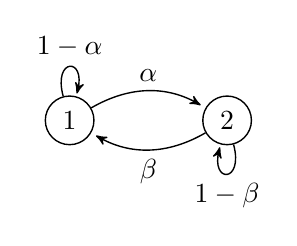
\begin{tikzpicture}[->,>=stealth',shorten >=2pt,line width=0.5pt,node distance=2cm]
            \node[circle,draw] (zero) {1};
            \node[circle,draw] (one) [right of=zero] {2};
            \path (zero) edge [loop above] node {\(1-\alpha \)} (zero);
            \path (zero) edge [bend left] node[above] {\(\alpha \)} (one);
            \path (one) edge [loop below] node {\(1-\beta \)} (one);
            \path (one) edge [bend left] node[below] {\(\beta \)} (zero);
        \end{tikzpicture}
    \end{center}
Thus, we can have say:
\[
    \mathbb{P} (X_3 = 1 | X_0 = 1, X_1 = 1 , X_2 - 2) = \beta 
\]

Another example that we can have is:
\[
    \mathcal{S} = \{1,2,3\} \quad \nu = (\nu_{1}, \nu_{2}, \nu_{3}) \quad \mathcal{P} = \begin{bmatrix}
        0 & 1 & 0 \\
        0 & \frac{1}{2} & \frac{1}{2}  \\
        \frac{1}{2} & 0 & \frac{1}{2} \\
    \end{bmatrix}
\]
    \begin{center}
        \begin{tikzpicture}[->,>=stealth',shorten >=2pt,line width=0.5pt,node distance=3cm]
            \node[circle,draw] (one) {1};
            \node[circle,draw] (two) [below right of=zero] {2};
            \node[circle,draw] (three) [below left of=zero] {3};
            \path (one) edge [bend left] node[below left] {\(1 \)} (two);
            \path (two) edge [bend left] node[above] {\(\frac{1}{2} \)} (three);
            \path (three) edge [bend left] node[below right] {\(\frac{1}{2} \)} (one);
        \end{tikzpicture}
    \end{center}
    given, \(\nu = (1,0,0)\), the outcomes of the Markov chain if we sample it are:
    \[
        \begin{aligned}
            X_n &= 1, 2, 3, 3, 1, 2, \dots \\
            &= 1, 2, 3, 1, 2, \dots \\ 
        \end{aligned}
    \] 
\end{example}
\vspace{1em}
Note that, to define the DTMC, we need the initial distribution, but the results wont change on the
choice of the distribution \(\nu\), assuming that the Markov chain is ergodic. Hence, while
defining the markov chain, the initial distribution is not mentioned, and can be assumed
arbitrarily.

\begin{theorem}[Necessary and Sufficient Conditions for DTSP to be Markov Chains]
    A DTSP \({(X_n)}_{n \geq 0}\) on \(\mathcal{S}\)  is a Markov chain \(\langle \mathcal{S} , \mathcal{P} 
    ,\nu \rangle\) if and only if:
    \[
        \mathbb{P} \left( 
            X_{n} = i_{n} , X_{n} = i_{n}, \dots, X_{0} = i_{0}
            \right) = \nu _{i_{0}} \mathcal{P} _{i_{0} i_{1}}
             \mathcal{P} _{i_{1} i_{2}} \dots \mathcal{P} _{i_{n-1} i_{n}} \quad \forall n \geq 0
    \] 
\end{theorem}
\begin{proof}
    To simplify the proof, assume that \(\mathcal{P}_{ij} > 0 \quad \forall i, j \in \mathcal{S} \).
    The theorem remains true in the general case, but requires more book-keeping.

    Suppose, \({(X_n)}_{n \geq 0}\) is a Markov chain \(\langle \mathcal{S} , \mathcal{P}
    , \nu \rangle\). 
    
    Using the fact,
    \[
        \begin{aligned}
            \mathbb{P}(A \cap B) &= \mathbb{P}(A) \mathbb{P}(B | A) \\
            \mathbb{P}(A \cap B \cap C) &= \mathbb{P}(A) \mathbb{P}(B | A) \mathbb{P}(C | A \cap B) \\
        \end{aligned}
    \]
    We get,
    \[
        \begin{aligned}
            \mathbb{P}(X_0 = i_0, \dots , X_n = i_n)  & = \mathbb{P} \left( 
                \{X_0 = i_0\} \cap \{X_1 = i_1\} \cap \dots \cap \{X_n = i_n\}
             \right)\\ 
             & = \mathbb{P}(X_0 = i_0) \mathbb{P}(X_1 = i_1 | X_0 = i_0) \dots \mathbb{P}(X_n = i_n | X_{n-1} = i_{n-1}) \\
             & = \mathbb{P} (X_0 = i_0) \mathbb{P}(X_1 = i_1 | X_0 = i_0) \dots \mathbb{P}(X_n = i_n | X_{n-1} = i_{n-1}) \\
             &\dots  \text{Using the memoeryless property of Markov chains} \\
                & = \nu _{i_0} \mathcal{P} _{i_0 i_1} \dots \mathcal{P} _{i_{n-1} i_n} \\
        \end{aligned}
    \]

    This proves the forward claim. To show the reverse claim:

    Put \(n=0\), in the claim, to trivially get the initial distribution back, showing one part of the definition.
    For the other part:
    \[
    \begin{aligned}    
        \mathbb{P}(X_{n} = i_{n} | X_{n-1} = i_{n-1}, \dots, X_{0} = i_{0}) &=
         \frac{\mathbb{P}(X_{n} = i_{n}, \dots, X_{0} = i_{0})}
         {\mathbb{P}(X_{n-1} = i_{n-1}, \dots, X_{0} = i_{0})} \\
         &= \frac{\nu _{i_0} \mathcal{P} _{i_0 i_1} \dots \mathcal{P} _{i_{n-1} i_n}}
         {\nu _{i_0} \mathcal{P} _{i_0 i_1} \dots \mathcal{P} _{i_{n-1} i_n}} \\
            &= \mathcal{P} _{i_{n-2} i_{n-1} } \\
    \end{aligned}
    \]

    Now we need to show:
    \[
        \mathbb{P}(X_{n} = i_{n} | X_{n-1} = i_{n-1})
    \]
    \[
        \begin{aligned}
            & = \frac{\mathbb{P}(X_{n-1} = i_{n-1}, X_{n} = i_{n})}{\mathbb{P}(X_{n-1} = i_{n-1})} \\
            & = \frac{\sum_{i_0 \in \mathcal{S} } \mathbb{P}(X_0 = i_0 \dots  X_{n-1} = i_{n-1}, X_{n} = i_{n})}
            {\sum_{i_0 \in \mathcal{S} } \mathbb{P}(X_{n-1} = i_{n-1}, X_{0} = i_{0})} \\
            & = \mathcal{P} _{i_{n-1} i_n} \\
        \end{aligned}
    \]
\end{proof}\vspace{1em}
In the above proof we have used the following series of fact:
\[
    \begin{aligned}
        \mathbb{P} (X_2 = j) & = \mathbb{P}(\Omega \cap \{X_2 = j\})\\
        &= \mathbb{P} \left[ 
            \bigcup_{i=1}^{ |S| } \{X_i = i\} \cap \{X_2 = j\}
         \right] \\
    \end{aligned}
\]
Using the fact:
\[
    (A \cup B) \cap C = (A \cap C ) \cup (B \cap C)
\]
we get:
\[
    \begin{aligned}
        \mathbb{P} (X_2 = j) & = \sum\limits_{i = 1}^{ |S| } 
        \mathbb{P} \left(
             X_i = i, X_2 = j
         \right)
    \end{aligned}
\]

\begin{theorem}[Markov Property]
    Let \({(X_n)}_{n \geq  0} \) be the markov chain detnoted by \(\langle \mathcal{S} ,\mathcal{P} ,\mu  \rangle \),
then condintional on \(\{X_m = i\}\), \(\{X_{m+n} \}\) is the markov chain \(\langle \mathcal{S} ,\mathcal{P} , \delta _i \rangle \) 
and is independent of \(X_1, X_2, \dots , X_m\), where \(\delta _i\) is the distribution that is 1 at \(i\)
 and 0 everywhere else, i.e
 \[
        \delta _i (j) \equiv \delta_{ij} =  \begin{cases}
            1 & \text{if } j = i \\
            0 & \text{otherwise} \\
        \end{cases} 
 \]
\end{theorem}
\begin{proof}
    It suffices to show the following, for any \(n \geq 0\) and on an event \(A\), related to \(X_0,\dots , X_m\):
    \[
        \begin{aligned}
            \mathbb{P} \left[ 
                (X_m = i_m, X_{m+1} = i_{m+1}, \dots , X_{m+n} = i_{m+n}) \cap A \mid X_m = i_m 
                \right] \\ 
                = \mathbb{P} ( A \mid X_m=i_m) \delta_{ij} \mathcal{P} _{i_m i_{m+1}} \dots 
                \mathcal{P} _{i_{m+n-1} i_{m+n}} 
            \end{aligned}
    \]
    The above equation is just conditional independence:
    \[
        \mathbb{P} (E_1 \cap  E_2 \mid X_m = i) = \mathbb{P} (E_1 \mid X_m = i) \mathbb{P} (E_2 \mid X_m = i)
    \]
    where \(E_2 = (X_m = i_m, X_{m+1} = i_{m+1}, \dots , X_{m+n} = i_{m+n})\) and \(E_1 = A\). The proof of the above statement goes as follows:

    Let \(A\) be an elementary event, i.e. \(A = \{X_0 = j_0, X_1 = j_1, \dots , X_m = j_m\}\). Consider the LHS of the above equation:
    Then, we have two cases:
    \begin{itemize}
        \item \textbf{Case 1}: \(j_m \neq i_m\). Then, the LHS is trivially 0, since \(A\) and \(E_2\) are disjoint.
        \item \textbf{Case 2}: \(j_m = i_m\). Then, we have further cases. When, \( i \neq i_m = j_m\), then 
        the LHS and RHS are again 0. But when \(i = i_m = j_m\), then the LHS is: 
        \begin{multline*}
        \begin{aligned}
                \mathbb{P} (
                    X_0 = j_0, X_1 = j_1, \dots X_m = j_m = i ,X_m = i_m = i, X_{m+1} = i_{m+1},\\ \dots , X_{m+n} = i_{m+n} \mid X_m = i_m = i 
                    )
                \end{aligned}
            \end{multline*}
            \[
                \begin{aligned}
                    &= \frac{\nu(j_o) \mathcal{P}_{j_0 j_1} \dots \mathcal{P}_{j_{m-1} j_m} 
                    \mathcal{P}_{j_m i_{m+1}} \dots \mathcal{P}_{i_{m+n-1} i_{m+n}}}
                    {\mathbb{P} (X_m = i_m = i)} \\
                    &= \frac{\mathbb{P} (A) \mathcal{P}_{i_m i_{m+1}} \dots \mathcal{P}_{i_{m+n-1} i_{m+n}}}
                    {\mathbb{P} (X_m = i_m = i)} \\
                    &= \mathbb{P} (A \mid X_m = i_m = i) \mathcal{P}_{i_m i_{m+1}} \dots \mathcal{P}_{i_{m+n-1} i_{m+n}} \\
                \end{aligned}
            \]
            \end{itemize}
    Thus, completing the proof. This can be extended to non elementary event \(A\) by using the fact that
    any event \(A\) can be written as a union of elementary events, i.e
    \[
        A = \bigcup_{i=1}^{ |S| } \{X_0 = i_0, X_1 = i_1, \dots , X_m = i_m\}
    \]
\end{proof}

\begin{theorem}[Linear Algebra and Markov Chains]
    Let \({(X_n)}_{n \geq 0}\) be the marrkov chain \(\langle \mathcal{S} , \mathcal{P} , \nu \rangle\).
    Then:
    \begin{enumerate}
        \item \(\mathbb{P} (X_n = j) = {(\nu \mathcal{P} ^{n})}_{j} \)
        \item \(\mathbb{P}_i (X_n = j) = \mathbb{P} \left( X_{m+n} = j \mid X_m = i \right) 
        = \mathcal{P}_{ij}^{(n)}\equiv \text{ij entry of } \mathcal{P} ^{n}\)
    \end{enumerate}
\end{theorem}
\begin{proof}
    The second statement is obivious from the first statement. The proof of the first statement goes as follows:

    \textbf{Proof by induction}: For \(n=0\), we have:
    \[
        \mathbb{P} (X_0 = j) = \nu _j \equiv \nu(j)  
    \]
    Now, assume that the statement is true for \(n\), then we have:
    \[
        \begin{aligned}
            \mathbb{P} (X_{n+1} = j) &= \mathbb{P} \left( 
                \bigcup_{i=1}^{ |S| } \{X_n = i , X_{n+1} = j\}
             \right) \\
                &= \sum_{i=1}^{ |S| } \mathbb{P} (X_n = i, X_{n+1} = j) \\
                &= \sum_{i=1}^{ |S| } \mathbb{P} (X_n = i) \mathbb{P} (X_{n+1} = j \mid X_n = i) \\
                &= \sum_{i=1}^{ |S| } \mathbb{P} (X_n = i) \mathcal{P}_{ij} \\
                &= \sum_{i=1}^{ |S| } {(\nu \mathcal{P}^n)}_j \mathcal{P}_{ij} \\
                &= {(\nu \mathcal{P}^{n+1})}_j \\
        \end{aligned}
    \]
\end{proof}

  
  % \part{Test}
\section{{Lecture Title}}

\subsection{Sub Section 1}
\label{sub_sec:sub_section_1}

\begin{theorem}
This is a theorem.
\end{theorem}
\begin{proof}
This is a proof.
\end{proof}
\begin{example}
This is an example.
\end{example}
\begin{explanation}
This is an explanation.
\end{explanation}
\begin{claim}
This is a claim.
\end{claim}
\begin{corollary}
This is a corollary.
\end{corollary}
\begin{prop}
This is a proposition.
\end{prop}
\begin{lemma}
This is a lemma.
\end{lemma}
\begin{question}
This is a question.
\end{question}
\begin{solution}
This is a solution.
\end{solution}
\begin{exercise}
This is an exercise.
\end{exercise}
\begin{definition}[Definition]
This is a definition.
\end{definition}
\begin{note}
This is a note.
\end{note}

% subsection sub_section_1 (end)

\newpage
  % \input{lectures/lec-02.tex}
  % \section{Todo Notes}

\todo[inline]{The original todo note withouth changed colours.\newline Here's another line.}
\lipsum[11]\unsure{Is this correct?}\unsure{I'm unsure about also!}
\lipsum[11]\change{Change this!}
\lipsum[11]\info{This can help me in chapter seven!}
\lipsum[11]\improvement{This really needs to be improved!\\What was I thinking?!}
\lipsum[11]\improvement[inline]{The following section needs to be rewritten!}
\lipsum[11]

\newpage

\lesson{Oct 20 2022 Thu (12:28:10)}{Graphs}

\noindent \begin{minipage}{0.53\textwidth}
    Lorem ipsum dolor sit amet, consetetur sadipscing elitr, sed diam nonumy eirmod
    tempor invidunt ut labore et dolore magna aliquyam erat, sed diam voluptua. At
    vero eos et accusam et justo duo dolores et ea rebum. Stet clita kasd gubergren,
    no sea takimata sanctus est Lorem ipsum dolor sit amet. Lorem ipsum dolor sit
    amet, consetetur sadipscing elitr, sed diam nonumy eirmod tempor invidunt ut
    labore et dolore magna aliquyam erat, sed diam voluptua. At vero eos et accusam
    et justo duo dolores et ea rebum. Stet clita kasd gubergren, no sea takimata
    sanctus est Lorem ipsum dolor sit amet.
\end{minipage}
\hspace{0.05\textwidth}
\begin{minipage}{0.4\textwidth}
  \vspace{1cm}
  \centering
  \incfig{limit-graph}
  \captionof{figure}{$y = g(t)$}
  \label{fig:limit_graph}
\end{minipage}

\newpage
  % end lectures
\end{document}